\documentclass[a4paper,12pt, italian]{book}
% \usepackage[a4paper]{geometry}
\usepackage[utf8x]{inputenc}
\usepackage[italian]{babel}

\usepackage[dvips]{graphicx}
\usepackage{latexsym}
\usepackage{amssymb}
\usepackage{color}
\usepackage{fancyhdr}
\usepackage{stmaryrd}
\usepackage{verbatim}
\usepackage{printlen}

%\usepackage{pstricks} %for dia macro images
%\usepackage{tikz}

\usepackage{listings} % for printing Java code
\lstloadlanguages{JAVA}
\lstset{
language=java,
basicstyle=\scriptsize,
aboveskip=1em,
belowskip=1em,
frame=TB,
tabsize=4,
}

\usepackage{pifont}     %for openstar in the title footnotes.
\usepackage[a4paper]{geometry}   %for margin settings.
\usepackage{fleqn}      %for left aligned equations.
\usepackage{txfonts}   
 %optional font package, if document is to be formatted with Times and compatible math fonts.
\usepackage{hyperref}   %optional packages if hyper linking is required in thedocument.
% the natbib package allows both number and author-year (Harvard)
% style referencing;
\usepackage{wasysym}
\usepackage{marvosym}
\usepackage{color}
\usepackage{subfigure}
\usepackage{eso-pic}


\newtheorem{definition}{Definition}[section]
%\newtheorem{example}[definition]{Example}
%\newtheorem{lemma}[definition]{Lemma}
%\newtheorem{theorem}[definition]{Theorem}
%\newtheorem{corollary}[definition]{Corollary}

\newenvironment{example}[1]%
{\refstepcounter{definition}%
{\medskip\noindent \emph{Example \thedefinition : #1}}.}%
{\medskip}

% MACROS
%%%%%%%% NOMI DEI CALCOLI E DEI LINGUAGGI %%%%%%%%%%%%%%%%%%%%%%%%%%
\newcommand{\wsc}{\textsc{ws-calculus}}
\newcommand{\wscalc}{\textsc{ws-calculus}} % alias
\newcommand{\tsbpel}{\textsc{tsBPEL}}
\newcommand{\mutsbpel}{\wsc} %re alias
\newcommand{\cows}{\textsc{\large cows}}
%\newcommand{\cows}{\textsc{c}\u{o}\textsc{ws}}
%\newcommand{\cows}{\textsc{COWS}}
\newcommand{\wsbpel}{\textsc{WS-BPEL}}
%\newcommand{\lwsbpel}{\wsbpel$_{\ell ight}$}

\newcommand{\blite}{\textsf{B}$\mathit{lite}$}
%\newcommand{\lwsbpel}{\textsf{B}lite}
%\newcommand{\lwsbpelll}{\textsf{Blite}}
%\newcommand{\lwsbpel}{\textsc{\large b}$_{\ell ite}$}
%\newcommand{\lwsbpel}{\textsc{S}$_{\ell ight}$}
%\newcommand{\lwsbpel}{\textsc{S}$_{\ell ite}$}
%\newcommand{\lwsbpel}{\textsc{B}$_{\ell ight}$}
\newcommand{\bpel}{\textsc{BPEL}}
\newcommand{\wsdl}{\textsc{WSDL}}
\newcommand{\xmlschema}{\textsc{XML} Schema}
\newcommand{\biz}{\textsc{Biztalk}}
\newcommand{\wscdl}{\textsc{WS-CDL}}
\newcommand{\pic}{$\pi$-calculus}
\newcommand{\Lpiclong}{localised $\pi$-calculus}
\newcommand{\Lpic}{L$\pi$}
\newcommand{\Klaim}{\textsc{Klaim}}
\newcommand{\orc}{Orc}


%%%%%%%%%%%%%%% SPAZI E SEPARATORI %%%%%%%%%%%%%%%%%%%%%%%%%%%
\newcommand{\quot}[2]{\begin{small} \begin{flushright}\begin{itshape} #1 \end{itshape}\\ #2 \end{flushright} \end{small}}
\newcommand{\spar}{\mid} % service parallel composition
\newcommand{\sepgr}{\!\quad | \quad\!} % separatore per le grammatiche
\newcommand{\arr}[1]{\langle #1 \rangle} %array: vanno esplicitamente messe le virgole
\newcommand{\set}[1]{\{#1\}} % parentesi per un insieme

%%%%%%%%%%%%%%%%% FUNZIONI %%%%%%%%%%%%%%%%%%%%%%%
\newcommand{\length}[1]{\mid\! #1 \!\mid} % lunghezza sostituzioni
\newcommand{\assoc}[2]{#1 \mapsto #2} % associazione variabile-valore

%%%%%%%%%%%%% PROOF %%%%%%%%%%%%%%%%%%%%%%%%%%

%%%%%%%%% PROOFTREE %%%%%%%%%%%%%%%%%%%%%%
\input{prooftree}

\newtheorem{Notation}{Notation}[section]

%\newcommand{\qed}%{\hfill\mbox{\ \vrule height4pt width3pt depth2pt}}
%  {\ \hbox{}\penalty10000\hfill$\Box$\medskip}
%
%\newenvironment{proof}%
%{\begin{trivlist}%
%\item[]{\it Proof.}
%}%
%{\qed
%\end{trivlist}
%}

%\newenvironment{proof}%
%{\vspace{-.5cm}%
%\begin{trivlist}%
%\item[]{\it Proof.}
%}%
%{\vspace{-.4cm}
%\qed
%\end{trivlist}
%}

\newenvironment{proofSketch}%
{\begin{trivlist}%
\item[]{\it Proof (sketch).}
}%
{\qed
\end{trivlist}
}

\newenvironment{observation}%
{\refstepcounter{definition}%
{\medskip\noindent \emph{Observation \thedefinition}}.}%
{\medskip}

\newcommand{\cvd}{\begin{flushright} $\Box$ \end{flushright}} % fine dimostrazione
%\newcommand{\cvd}{\begin{flushright} $\Box$ \end{flushright}} % fine dimostrazione

%%%%%%%%%%%%%%%%%% COSTANTI %%%%%%%%%%%%%%%%%%%%%
\newcommand{\define}{\triangleq} % notazione per assegnare un nome a vari termini del calcolo
\newcommand{\undef}{\mathbf{undef}} % denota undefined
\newcommand{\false}{\mathbf{false}}
\newcommand{\true}{\mathbf{true}}
\newcommand{\und}{\_} % simbolo underscore


%%%%%%%% TABELLE %%%%%%%%%%%%%%%%%%%%%%%%%%
%\newcommand{\etich}[2]{#1 \quad #2}
\newcommand{\etich}[2]{
\begin{array}{l}
#2 \\ #1
\end{array}}

\newcommand{\rulelabel}[1]{\textrm{\footnotesize{(#1)}}}
%\newcommand{\rulelabel}[1]{\textrm{\small{(#1)}}}



\def \overstackrel#1#2{\mathrel{\mathop{#1}\limits^{#2}}}

\newcommand{\delimite}[1]{\mbox{$\overstackrel{\belowfill}{\mbox{$\overstackrel{\quad #1 \quad}{\abovefill}$}}$}}
%\newcommand{\delimite}[1]{\mbox{$\overstackrel{\belowfill}{\mbox{$\overstackrel{ \ #1 \ }{\abovefill}$}}$}}

\makeatletter
\def \abovefill{
  {\vrule width0.3mm height 1.8mm depth-0.3mm}
  \leaders\hrule height1.8mm depth-1.5mm\hfill
  {\vrule width0.3mm height 1.8mm depth-0.3mm}}
\makeatother

\makeatletter
\def \belowfill{
  {\vrule width0.3mm height1.5mm}
  \leaders\hrule height0.3mm\hfill
  {\vrule width0.3mm height1.5mm}}
\makeatother




%%%%%%%%% FRECCE %%%%%%%%%%%%%%%%%%%%%%
\makeatletter
\def \rightarrowfill{\m@th\mathord{\smash-}\mkern-6mu%
  \cleaders\hbox{$\mkern-2mu\mathord{\smash-}\mkern-2mu$}\hfill
  \mkern-6mu\mathord\rightarrow}
\makeatother

\makeatletter
\def \Rightarrowfill{\m@th\mathord{\smash=}\mkern-6mu%
  \cleaders\hbox{$\mkern-2mu\mathord{\smash=}\mkern-2mu$}\hfill
  \mkern-6mu\mathord\Rightarrow}
\makeatother

\makeatletter
\def \OrcRightarrowfill{\m@th\mathord{\smash\vDash\!\!\!=}\mkern-6mu%
  \cleaders\hbox{$\mkern-2mu\mathord{\smash=}\mkern-2mu$}\hfill
  \mkern-6mu\mathord\Rightarrow}
\makeatother


\makeatletter
\def \nrightarrowfill{\m@th\mathord{\smash-}\mkern-6mu%
  \cleaders\hbox{$\mkern-2mu\mathord{\smash-}\mkern-2mu$}\hfill
  \mkern-6mu\mathord\nrightarrow}
\makeatother

\newcommand{\tsarrow}[1]{\overstackrel{\rightarrowfill}{\ \ #1\ \ }}
\newcommand{\Tsarrow}[1]{\overstackrel{\Rightarrowfill}{\ \ #1\ \ }}
\newcommand{\ntsarrow}[1]{\overstackrel{\nrightarrowfill}{\ \ #1\ \ }}

\newcommand{\tsarrowtau}{\tsarrow{\scoml{\single{n}}{\emptyset}{\arr{\tau}}{\arr{\tau}}}}
\newcommand{\OrcTsarrow}[1]{\overstackrel{\OrcRightarrowfill}{\ \ #1\ \ }}


%%%%%%%%% FRECCE WSC %%%%%%%%%%%%%%%%%%%%%%

\makeatletter
\def \rightarrowfillN{\m@th\mathord{\smash-}\mkern-6mu%
  \cleaders\hbox{$\mkern-2mu\mathord{\smash-}\mkern-2mu$}\hfill
  \mkern-6mu\mathord \not \rightarrow}
\makeatother
\newcommand{\tsarrowN}[1]{\overstackrel{\rightarrowfillN}{\ \ #1\ \ }}

\newcommand{\redarrow}[1]{\mbox{$\succ\!\overstackrel{\rightarrowfill}{\ \ #1\ \ }$}}
\newcommand{\redarrowN}[1]{\succ\!\overstackrel{\rightarrowfillN}{#1}}
\newcommand{\notRedarrowErr}{\succ\!\not\rightarrow^{err}}

%%%%%%%%% FRECCE WSBPEL %%%%%%%%%%%%%%%%%%%%%%

\makeatletter
\def \bpelrightarrowfill{\m@th\mathord{\smash-}\mkern-6mu%
  \cleaders\hbox{$\mkern-2mu\mathord{\smash-}\mkern-2mu$}\hfill
  \mkern-6mu\mathord\rightarrowtriangle}
\makeatother

\newcommand{\bpeltsarrow}[1]{\overstackrel{\bpelrightarrowfill}{\ \ #1\ \ }}

\newcommand{\bpelredarrow}[1]{\succ\!\overstackrel{\bpelrightarrowfill}{\ \ #1\ \ }}

\makeatletter
\def \nRightarrowfill{\m@th\mathord{\smash=}\mkern-6mu%
  \cleaders\hbox{$\mkern-2mu\mathord{\smash=}\mkern-2mu$}\hfill
  \mkern-6mu\mathord\nRightarrow}
\makeatother

\newcommand{\nTsarrow}[1]{\overstackrel{\nRightarrowfill}{\ \ #1\ \ }}

\definecolor{back}{gray}{1}
\definecolor{rcv}{gray}{0.9}
\definecolor{inv}{gray}{0.9}
\definecolor{cnd}{gray}{0.5}
\definecolor{ass}{gray}{0.8}
\definecolor{cor}{gray}{0.5}

\definecolor{Mygray}{gray}{0.75}

%\definecolor{mygray}{gray}{0.45}
%\newcommand{\xmod}[1]{\textcolor{blue}{#1}} % BPEL SAT

\newcommand{\modif}[1]{\textcolor{red}{#1}} % BPEL SAT

\newcommand{\mylemma}[2]{
\vspace{4mm}\noindent{\bf Lemma~#1.}
{\it #2 }
\vspace{4mm}
}

\newcommand{\oracle}{Oracle BPEL}
\newcommand{\xnew}{\marginpar{new!}}

\newcommand{\plrec}{\ell^{\,r}}
\newcommand{\plinv}{\ell^{\,i}}

%%%%%%%%% BPEL FONTS %%%%%%%%%%%%
%\newcommand{\xbpel}[1]{\texttt{<#1>}} % BPEL XML FONT
%\newcommand{\xlbpel}[1]{\texttt{<#1}} % BPEL XML left FONT
%\newcommand{\xrbpel}[1]{\texttt{#1>}} % BPEL XML right FONT
%\newcommand{\xzbpel}[1]{\texttt{#1}} % BPEL XML no <> FONT
\newcommand{\x}[1]{{\sf #1}} % BPEL GENERAL FONT
\newcommand{\xcmd}[1]{{\sf #1}} % BPEL GENERAL COMMAND FONT
\newcommand{\xx}{\x{x}} % BPEL VARIABLE
\newcommand{\xy}{\x{y}} % BPEL VARIABLE
\newcommand{\xz}{\x{z}} % BPEL VARIABLE
\newcommand{\xo}{\x{o}} % BPEL OPERATION
\newcommand{\xp}{\x{p}} % BPEL PARTNER
\newcommand{\xq}{\x{q}} % BPEL PARTNER
\newcommand{\xe}{\x{e}} % BPEL EXP
\newcommand{\xv}{\x{v}} % BPEL VALUE
\newcommand{\xw}{\x{w}} % BPEL VARIABLE/VALUE
\newcommand{\xu}{\x{u}} % BPEL VARIABLE/PARTNER
\newcommand{\xid}{\x{s}} % SCOPE ID
\newcommand{\xb}{\x{b}} % business process
\newcommand{\xs}{\x{a}} % SERVICE ACTIVITIES
\newcommand{\xsc}{\x{a}_{s}}
\newcommand{\xsa}{\x{r}} % START ACTIVITIES
%\newcommand{\xh}{\x{h}} % HANDLERS
\newcommand{\xh}{\xs} % HANDLERS
\newcommand{\xsla}{\x{sh}}
\newcommand{\xa}{\x{b}} % BASIC ACTIVITY
\newcommand{\xd}{\x{d}} % DEPLOYMENT
\newcommand{\xI}{\x{s}} % INSTANCE
\newcommand{\xcorr}{\x{c}} % CORRELATION VARIABLES
\newcommand{\xl}[1]{\dot{#1}} % LINK VARIABLE
\newcommand{\xfs}[1]{\mathcal{S}_{#1}} % TOP LEVEL SCOPE IDENTIFIERS
\newcommand{\xcs}[2]{\mathcal{C}^{\,#1}_{#2}} % SCOPE IDENTIFIERS ARGS of CMP
\newcommand{\xC}[1]{\mathcal{H}(#1)} %
\newcommand{\xDC}[3]{\mathcal{D}\mathcal{C}(#1, #2, #3)} %
\newcommand{\xell}{\single{\ell}} % LOCK
%%% extra label
\newcommand{\talpha}{t}
\newcommand{\oalpha}{!\,\talpha}
\newcommand{\ialpha}{?\,\talpha}
%%%%%%%%%%% SEPARATORI %%%%%%%%%%%%%%%%%%%%%%%%
\newcommand{\xmid}{\,,\,} % separatore componenti: istanze e specifiche
%\newcommand{\xspar}{\spar} % separatore deployments
\newcommand{\xspar}{\|\,} % separatore deployments
\newcommand{\xdisj}{,} % union of states with disjoint domains
\newcommand{\xupd}{\circ} % state updating
\newcommand{\xxdef}{\stackrel{_{def}}{=}} % definition

%%%%%%%%%%% STRUCT EQUIV %%%%%%%%%%%%%%%%%%%%%%%%
%\newcommand{\xequiv}{\stackrel{\textrm{\tiny bpel}}{\equiv}}
\newcommand{\xequiv}{\equiv}
%%%%%%%%%%% TRUE FALSE %%%%%%%%%%%%%%%%%%%%%%%%
\newcommand{\xfalse}{\x{ff}}
\newcommand{\xtrue}{\x{tt}}
\newcommand{\xunset}{\x{null}}
\newcommand{\unspec}{\bot} % UNSPECIFIED
\newcommand{\xnok}{\x{ff}}
\newcommand{\xok}{\x{tt}}
\newcommand{\mybackslash}{-} %

%%%%%%%%% BPEL ACTIVITIES %%%%%%%%%%%%
% BASIC
\newcommand{\xcomm}[1]{\textit{\% #1}}
%\newcommand{\xrec}[3]{\xcmd{rcv}(#1,#2,#3)}
\newcommand{\xrec}[3]{\xcmd{rcv}\,#1\, #2\, #3}
\newcommand{\xinv}[3]{\xcmd{inv}\,#1\,#2\,#3}
%\newcommand{\xinv}[3]{\xcmd{inv}(#1,#2,#3)}
%\newcommand{\xmsg}[3]{\xcmd{!}\,\xapp{#1}{\xapp{#2}{#3}}}
\newcommand{\xmsg}[3]{\ll\!\xapp{#1}{\xapp{#2}{#3}}\!\gg}
%\newcommand{\xreca}[3]{\xcmd{rcv}\arr{#1,#2,#3}}
%\newcommand{\xinva}[3]{\xcmd{inv}\arr{#1,#2,#3}}
%\newcommand{\xinvs}[4]{\xcmd{inv}(#1,#2,#3,#4)}
\newcommand{\xass}[2]{#1 := #2}
\newcommand{\xassv}[2]{#1 \leftarrow #2}
%%
\newcommand{\xthr}{\xcmd{throw}}
\newcommand{\xexit}{\xcmd{exit}}
\newcommand{\xskip}{\xcmd{empty}}
\newcommand{\xstop}{\xcmd{stop}}
%%
%% SMALL
\newcommand{\xsthr}{\mbox{\small{\textsf{throw}}}}
\newcommand{\xsexit}{\mbox{\small{\textsf{exit}}}}
\newcommand{\xsskip}{\mbox{\small{\textsf{empty}}}}
\newcommand{\xsstop}{\mbox{\small{\textsf{stop}}}}
\newcommand{\xshalt}[1]{\mbox{\small{\textsf{end}}}(#1)}
%%
\newcommand{\recsep}{\xsucc} % BPEL MOD
%\newcommand{\xsexit}{\textsf{\small exit}}
%\newcommand{\xsthr}{\textsf{\small thr}}
\newcommand{\xcmpscope}[1]{\xcmd{cmpsc}(#1)}
%\newcommand{\xcmp}[1]{\xcmd{cmp}(#1)}
\newcommand{\xcmpa}[2]{\xcmd{cmp}(#1,#2)}
\newcommand{\xattr}{\Diamond}%{\diamond}
\newcommand{\xattrscope}{\Diamonddot}%{!}
\newcommand{\xattrall}{\Diamondblack}%{\ast}
\newcommand{\xattrt}{\blacktriangledown}
%\newcommand{\xemp}{\x{skip}}
%\newcommand{\xskip}{\xcmd{empty}}
%\newcommand{\xstop}{\mbox{\textsf{\small stop}}}
% STRUCTURED
\newcommand{\xsucc}{\, ; }
\newcommand{\xpar}{\,|\,}
\newcommand{\xplus}{\,+\,}
%\newcommand{\xif}[3]{\x{if}(#1)\, \x{then}\, \{ #2 \}\, \x{else}\, \{#3\}}
%\newcommand{\xifs}[2]{\x{if}(#1)\, \x{then}\, \{ #2 \}}
\newcommand{\xif}[3]{\xcmd{if}(#1)\{ #2 \}\{#3\}}
\newcommand{\xifs}[2]{\xcmd{if}(#1)\{ #2 \}}
\newcommand{\xwhile}[2]{\xcmd{while}(#1)\, \{ #2\}}
\newcommand{\xpick}{{\displaystyle \sum_{i\in I}\xrec{\tilde{\xu}_i}{\xo_i}{\bar{\xx}_i}\recsep\xs_i}}
\newcommand{\xpicknodisplay}{\sum_{i \in I}\xrec{\tilde{\xu}_i}{\xo_i}{\bar{\xx}_i}\recsep\xs_i}
\newcommand{\xpicknoemph}{\sum_{i \in I,I\neq\emptyset}\xrec{\tilde{\xu}_i}{\xo_i}{\bar{\xx}_i}\recsep\xs_i}
\newcommand{\xtarget}[3]{\{#2\}\stackrel{#1}{\Rightarrow} #3}
\newcommand{\xsource}[2]{#1 \Rightarrow\{#2\}}
%\newcommand{\xscopeh}[2]{[\![\,#2 \,]\!]_{#1}}
%\newcommand{\xscopeh}[2]{\lbag\,#2 \,\rbag_{#1}}
%\newcommand{\xscope}[4]{[#2 \bullet #3 \star #4]_{#1}}
%\newcommand{\xscopec}[3]{[#2 \star #3]_{#1}}
%\newcommand{\xscopef}[3]{[#2 \bullet  #3]_{#1}}
%\newcommand{\xscopez}[2]{[#2]_{#1}}
%\newcommand{\xscopeh}[2]{\lbag\,#2 \,\rbag_{#1}}
%\newcommand{\xscope}[4]{[#2 \bullet #3 \star #4]}
\newcommand{\xscope}[4]{[#1 \bullet #2 \star #3\, \triangle\, #4]}
\newcommand{\xscopecd}[3]{[#1 \star #2 \, \triangle\, #3]}
\newcommand{\xscopefd}[3]{[#1 \bullet #2 \, \triangle\, #3]}
\newcommand{\xscopef}[2]{[#1 \bullet #2]}
\newcommand{\xscopec}[2]{[#1 \star #2]}
\newcommand{\xscoped}[2]{[#1 \, \triangle\, #2]}
\newcommand{\xscopefc}[3]{[#1 \bullet #2 \star #3]}
\newcommand{\xscopez}[1]{[#1]}
\newcommand{\xdl}{\x{done}}
\newcommand{\xsuml}{\x{pick}}
%\newcommand{\xdl}{\x{done}}
\newcommand{\xproc}[2]{\xscopef{#1}{#2}}
%\newcommand{\xprot}[2]{\textcolor{green}{\llparenthesis #1\rrparenthesis_{#2}}} % handler
\newcommand{\xprot}[1]{\llparenthesis #1\rrparenthesis} % handler
%%%%%%%%%%%%%%%% DEPLOY %%%%%%%%%%%%%%%%%%
\newcommand{\xnet}[1]{\{\, #1 \,\}}
\newcommand{\xeng}[2]{\{ #1 \}_{#2}}
\newcommand{\xinst}[2]{#1 \vdash #2 }
\newcommand{\xinstnostate}[2]{#2}
\newcommand{\xnoCONF}[4]{#2\!\Downarrow^{#1,#4}_{#3}}
\newcommand{\noexit}[1]{#1\!\Downarrow_{\xexit}}
\newcommand{\nothr}[1]{#1\!\Downarrow_{\xthr}}
\newcommand{\noexitthr}[1]{#1\!\Downarrow_{\xexit/\xthr}}
\newcommand{\xnullinst}{\xinst{\xsigma}{\xskip/\xstop}}
\newcommand{\xemptycorr}{\emptyset} % empty correlation set
\newcommand{\xcorrset}[1]{\{#1\}}
%%%%%%%%%%%%%%%% LABELS %%%%%%%%%%%%%%%%%%
\newcommand{\xalpha}{\alpha}
\newcommand{\xnum}{n}
\newcommand{\xtau}{\tau}
%\newcommand{\xrecl}[3]{?(#1, #2, #3)}
\newcommand{\xrecl}[3]{?\,\xapp{#1}{\xapp{#2}{#3}}}
\newcommand{\xassl}[2]{#1 \leftarrow #2}
\newcommand{\xcoml}[1]{\tau( #1 )}
%\newcommand{\xinvl}[3]{!(#1, #2 , #3)}
\newcommand{\xinvl}[3]{!\,\xapp{#1}{\xapp{#2}{#3}}}
\newcommand{\xmsgl}[3]{!\,\xapp{#1}{\xapp{#2}{#3}}}
%\newcommand{\xcmpl}[1]{\stackrel{\curvearrowleft}{_#1}}
%\newcommand{\xdonel}[1]{\checkmark_{\!#1}}
\newcommand{\xdonel}[1]{(#1)}
%\newcommand{\xthrl}[1]{\Rsh_{\!#1}}
\newcommand{\xthrl}{\Rsh}
\newcommand{\xexitl}{\boxast}
%%%%%%%%%%%%%%%%%%%%% MATCH %%%%%%%%%%%%%%%%%%%%%
\newcommand{\xxnewmatch}[4]{\x{match}(#1,\, #2,\, #3,\, #4)}
\newcommand{\xapp}[2]{#1\! : \! #2}
%\newcommand{\xhalt}[1]{\x{terminate}(#1)}
\newcommand{\xhalt}[1]{\x{end}(#1)}
\newcommand{\xencod}[1]{\langle\!\langle#1\rangle\!\rangle}
\newcommand{\xencodi}[2]{\langle\!\langle#1\rangle\!\rangle_{#2}}
\newcommand{\xencodii}[3]{\langle\!\langle#1\rangle\!\rangle_{#2, #3}}
\newcommand{\xencodiii}[4]{\langle\!\langle#1\rangle\!\rangle_{#2, #3, #4}}
%\newcommand{\xencodiv}[7]{\langle\!\langle#1\rangle\!\rangle_{#2, #5,#6}^{#3, #4,#7}}
%\newcommand{\xencodiv}[7]{\langle\!\langle#1\rangle\!\rangle_{#2, #5}^{#3, #4,#7}}
\newcommand{\xencodiv}[7]{\langle\!\langle#1\rangle\!\rangle_{#2, #5}^{#3, #4}}
\newcommand{\xdom}[1]{dom(#1)}
\newcommand{\xvars}[1]{V(#1)}
\newcommand{\xsigma}{\x{\mu}}
\newcommand{\xddot}[2]{{#2}_{#1}^{\xattrall}}
\newcommand{\xdddot}[2]{{#2}_{#1}^{\xattrscope}}
\newcommand{\xenv}[1]{\{#1\}}
%\newcommand{\xddotsigma}{\ddot{\sigma}}
\newcommand{\updat}[2]{\xenv{\assoc{#1}{#2}}}
\newcommand{\xupdat}[3]{\xenv{\xassoc{#1}{#2}{#3}}}
\newcommand{\xassoc}[3]{#2 \stackrel{_{#1}}{\mapsto} #3}
\newcommand{\xall}[3]{\mathcal{D}(#1, #2, #3)}
\newcommand{\xS}{\mathcal{S}}
%\newcommand{\xT}{\mathcal{T}}
\newcommand{\xdone}{\hat{d}}
%%% TERMINATION SIGNALS
%\newcommand{\xtexit}{\hat{t}_{exit}}
%\newcommand{\xtthr}{\hat{t}_{thr}}
\newcommand{\xterm}[3]{\mathcal{T}_{\!\!#1,#2}^{#3}} % termination handler
\newcommand{\comple}{\hat{c}}
\newcommand{\xhand}{\hat{h}}
\newcommand{\xkill}{\hat{k}}
\newcommand{\xdot}{\x{\cdot}}
%%%%%%%%%%%%%%%%%% QUEUE %%%%%%%%%%%%%%%%%%%%%%%
\newcommand{\xqq}{\mathtt{q}}
\newcommand{\queue}{\mathit{Q}}
\newcommand{\xins}{\op_{ins}}
\newcommand{\xdel}{\op_{rem}}
%%%%%%%%%%%%%%%% EQUIVALENCE %%%%%%%%%%%%%%%%%%%%
\newcommand{\opeq}[2]{#1 \opeqs #2}
\newcommand{\opeqs}{\stackrel{\textrm{\tiny bpel}}{\approx}}
%\newcommand{\opeqs}{\stackrel{\text{\tiny bpel}}{\approx}}
%\newcommand{\opsims}{\stackrel{\text{\tiny bpel}}{\leq}}
\newcommand{\opsims}{\stackrel{\textrm{\tiny bpel}}{\leq}}
%\newcommand{\opeqs}{\sim_{\x{bpel}}}
%\newcommand{\opsims}{\leq_{\x{bpel}}}
\newcommand{\opsim}[2]{#1 \opsims #2}




%%% SHIPPING EXAMPLE %%%%%%%

\newcommand{\xitcc}{items}
\newcommand{\xitc}{shipped}
\newcommand{\complete}{c}
\newcommand{\id}{id}
\newcommand{\itemsTot}{items}
\newcommand{\itemsCount}{count}
\newcommand{\shipPriceCalc}{priceCalc}
\newcommand{\shipPriceComp}{comp}


\pagestyle{fancy}

% i comandi seguenti impediscono la scrittura in maiuscolo
% dei nomi dei capitoli e dei paragrafi nelle intestazioni
\renewcommand{\chaptermark}[1]{\markboth{#1}{}}
\renewcommand{\sectionmark}[1]{\markright{\thesection\ #1}}
\fancyhf{} % rimuove l’attuale contenuto dell’intestazione
            % e del pi\‘e di pagina
\fancyhead[LE,RO]{\bfseries\thepage}
\fancyhead[LO]{\bfseries\rightmark}
\fancyhead[RE]{\bfseries\leftmark}
\renewcommand{\headrulewidth}{0.5pt}
\renewcommand{\footrulewidth}{0pt}
\addtolength{\headheight}{0.5pt} % riserva spazio per la linea
\fancypagestyle{plain}{%
   \fancyhead{} % ignora, nello stile plain, le intestazioni
   \renewcommand{\headrulewidth}{0pt} % e la linea
}


\newcommand{\mnote}[1]{%
  \marginpar[{\raggedleft \footnotesize \sffamily  \textcolor{red}{#1}\\}]{
    {\raggedright \footnotesize \sffamily  \textcolor{red}{#1} \\}}}

\newcommand{\icode}[1]{\textsf{#1}}

\newcommand{\logo}[1]{\AddToShipoutPicture*{\AtPageCenter
{\makebox(0,0){\centering \includegraphics[width=0.8\paperwidth]{#1}}}}}
%\newtheorem{deff}{Definizione}
%\newtheorem{es}{Esempio}
%\newtheorem{pro}{Proposizione}
%\newtheorem{thm}{Teorema}
%\newtheorem{lem}{Lemma}

\linespread{1.2}
\setlength{\topmargin}{20pt}
\setlength{\textheight}{620pt}
%\setlength{\hoffset}{50pt}
\setlength{\evensidemargin}{10pt}
\setlength{\oddsidemargin}{40pt}
%\setlength{\rightsidemargin}{20pt}

\begin{document}
\hyphenation{e-se-guir-li ese-cu-zio-ne rap-pre-sen-ta-zio-ne de-fi-ni-sco-no
co-min-cias-se a-spet-ti si-mu-la-re se-con-do an-dia-mo sta-ti-ca}
\sloppy

\title{\textsf{ \textbf{Realizzazione di un motore d'esecuzione per un
  linguaggio di orchestrazione di servizi} \\ 
  \em \large Blite ovvero BPEL in versione lite}\\ } 
  \author{Paolo Panconi}
 
% \uselengthunit{pt}
% \printlength{\textwidth}
% \printlength{\textheight}
%\abstractract{Tesi di Laura di Paolo Panconi \ldots}
\maketitle
%\thispagestyle{empty}
\begin{figure}
\begin{center}
%\includegraphics[width=0.8 in, height= 0.8 in]{stemma2000bn.eps}
\end{center}
\end{figure}
\begin{center}
{\LARGE\bf{Universit\`a degli Studi di Firenze}}\\
\vskip 0.5cm
{\Large Facolt\`a di Scienze Matematiche, Fisiche e Naturali}\\
\medskip
{\Large Corso di Laurea in Matematica }\\
\vskip 0.3cm
{\large Anno Accademico 2001 - 2002}\\
\vskip 0.3cm
{\large Tesi di Laurea}\\
\vspace{1.1cm}
{\Huge\bf{Fisiopatologia della}}\\
\vskip 4.2mm
{\Huge\bf{Trombopoiesi e}}\\
\vskip 4.2mm
{\Huge\bf{Modellizzazione Matematica}}\\
\vspace{0.7 cm}
\end{center}
\begin{center}
{\large\bf{Laureanda:}}\\
\vspace{ 2mm}
{\Large{Francesca Di Patti}}\\
\vspace{1.7 cm}
{\large\bf{Relatore:}}\\
\vspace{2mm}
{\Large Prof. Luigi Brugnano}\\
\vspace{1.7 cm}
{\large\bf{Correlatore:}} \hspace{4.7cm} {\large\bf{Correlatore:}}\\
\vspace{2mm}
{\Large{Prof. Mario Primicerio}}
 \hspace{\stretch{1}} {\Large{Dott. Giovanni Longo}}\\
\end{center}
 % frontespizio
\newpage

\tableofcontents

\listoffigures
\listoftables

% Introduzione
%\include
%\input
%{intro/intro}

% Intro
\include
%\chapter{Un'introduzione a SOA e ai Servizi Web}

% Linguaggi BPEL e Blite
\include
%\chapter{Il linguaggio per l'orchestrazione}

\section{BPEL, lo standard per l'orchestrazione di Servizi Web}
Abbiamo visto come SOA e i Servizi Web siano una delle risposte più recenti
alla necessità di integrare funzionalità applicative eterogenee, e di fornire
un modello di sviluppo software che sia il pi\`u efficace possibile rispetto
alla natura dinamica dei domini applicativi tipici delle grandi realtà
aziendali.

Alla base della metodologia SOA vi è l'approccio ``bottom-up'', secondo cui è
possibile comporre le funzionalita di base offerte dalle diverse applicazioni
aziendali per crearne di più complesse e articolate. Gli standard e i linguaggi
dei Web Services foniscono il supporto tecnologico e formale per realizzare tale
integrazione che nella maggior parte degli scenari reali prevede di dover far
comunicare tecnolgie e formalismi del tutto eterogeni e incopatibli. Uno delle
possibilità più interessanti è quella di poter utilizzare il patrimonio storico
(``legacy'') del software azzindale tramite standard moderni e aperti, e poter
fare dialogare le applicazioni di ultima generazione con quelle più ``mature'',
che spesso mantengono un alto valore aziendale ma si basano su tecnologie e
metodologie proprietarie ormai difficilmente manutenibili.

Predisporre i componenti e renderli disponibili secondo il paradigma della
Architettura Orientata ai Servizi certo non realizza tutte le necessità di un
complesso sistema aziendale, il passo successivo non può essere che quello di
comporre le singole funzionalità di base per realizare i flussi operativi che
implemetano le reali politiche e strategie di business. Le attività aziendali
quindi possono essere rappresentate come processi (``Business Process'') che
raggruppano le singole funzionalità secondo precise regole aziendali (``Business
Rules'') e tramite primitive di aggregazione che attuano dipendeze temporali e
logiche fra i diversi componenti publicati come servizi (``Service
Orchestration''). Se si può pensare che le singole funzionalità siano i mattoni
del business e che abbiano una certa robustezza temporale, in termini di
specifica e implemetazione, i processi al contrario possono essere fortemente
dinamici e mutevoli, per poter facilmente adeguarsi alle necessità sempre nuove
che si presentano nelle attività di un'azienda.

Si capisce quindi come nasca la necessità di un formalismo specifico per la
definizione e realizzazione di tali processi. In generale si vorrebe poter
disporre di un linguaggio semplice e flessibile che possa essere utilizzato a
diversi livelli aziandali, compreso e adoperato dalle diverse figure
professionali che partecipano alla definizione e attuazione dei processi
stessi. Si vorrebbe disporre non solo di un linguaggio di programmazione
utile ai tecnici del software ma anche di un formalsmo usabile dai manager e
dagli esperti dei domini applicativi, che potese realizzare una piattaforma comune
per la collaborazione fra le diverse arie disciplinari.

E' proprio come risposta a tale necessità che si propone BPEL, un linguaggio
basato su XML per la definizione di processi aziendali realizzati come
composizione di funzionalità esposte da Servizi Web. BPEL storicamente nasce
dalla fusione di due teconlogie sviluppate indipendetemente all'inizio degli
anni 2000: WSFL (Web Service Flow Language) di IBM e XLANG di Microsoft. La
prima versione del linguaggio (BPEL4WS ``Business Process Execution Language for Web Services - Version 1.0'')
risale al 31 Luglio 2002 e fu prodotta del lavoro congiuto di grandi
aziende come IBM, BEA, SAP, Siebel e Microsoft. Dall'Aprile del 2003 il lavoro
di stesura della versione successiva (1.1) è stato affidato alla supervisione di
OASIS, società nata con il compito di realizzare standard aperti e condivisi
dalla comunità internazionale, al 5 Maggio 2003 è datato il rilascio di questa
versione nella stesura ufficiale. Oasis è  anche la curatrice della
versione 2.0 dello standard (WS-BPEL ``Web Services Business Process Execution
Language Version 2.0'') che ha visto il primo rilascio ufficiale in data
11 Aprile 2007.
\\
\ldots
\newpage

Nonostante BPEL sia ampiamente documentato da specifiche e standard ufficiali e
sia disponibile in diverse implemetazioni, le problematiche realitive al suo
uso non mancano e alcune di esse possono essere attribuite alla
mancanza di una semantica formale. Il processo di realizzazione di applicazioni BPEL
risulta difficile e fortemente soggetto ad errori anche per la presenza di
costrutti complessi come: il parallelismo, la concorrenza, la terminazione
forzata di attività, la correlazione e la compensazione, quest'ultima utilizzata
per la realizzazione di ``Long-Running Transaction'', e forse ancora non 
compresa in tutti i suoi aspetti e potenzialità dagli utilizzatori. In tal
senso si è pensato che un processo di analisi e di formalizzazione di
tali costrutti potesse essere utile sia per chi si trova ad utilizzarli sia per
coloro che ne definiscono le specifiche in linguaggio naturale, in modo tale da
renderne più chiaro e eventualmente semplificarne gli aspetti più delicati.

Un approccio, per cercare di affrontare queste problematiche, è stato quello di
utilizzare la teoria dei metodi formali e delle algebre di processo per la
definizione di una sematica formale e per la realizzazione successiva di una
piattaforma per la verifica e la dimostrazione di proprietà di applicazioni
basate su BPEL. Con tale scopo è stato creato Blite, una variante semplificata di
BPEL, che riproduce alcune delle sue funzionalità più caratteristiche cercando
d'altra parte di semplificarne alcuni aspetti ritenuti marginali nella
realizzazione del modello Process Orinted.
   
Il lavoro svolto in questa tesi è da considerarsi a supporto di questa attività,
come un ulteriore verifica e confronto del processo di astrazione teorica e
formale con gli aspetti più concreti e tecnologici legati all'implementazione di
un linguaggio come BPEL per l'orchestrazione distribuita di servizi. Infatti
l'obiettivo primario è stato quello di realizzare un'implemetazione di Blite che
potesse essere il più vicino possibile, per caratteristiche e applicabilità, ai
motori di esecuzione di BPEL attualmente disponibili. Se da un lato Blite vuole
essere un'analisi di BPEL fatta tramite un processo di astrazione e
formalizzazione, il lavoro qui esposto vuole essere a sua volta un'analisi di
tale processo, nel senso che ne vuole verificare la compatibilità e l'attinenza
con le problematiche più concrete e tecnologiche presenti nell'ambito della
orchestrazione di servizi. Di fatto quello che abbiamo fatto non è altro che un
test critico di come i costrutti formali utilizzati per fornire la semtica del
liguaggio, potessero essere realmente implementati in scenari di sowfware di
produzione, e che quindi continuassero a mantenere un legame a doppio filo con
il mondo delle tacnologia da cui hanno tratto iniziale ispirazione.
\\

Di seguito andremo a decrivere la sintassi e  la sematica originali di Blite e
le versioni leggermente modificate di cui è stata realizzata l'implementazione.

%%%%%%%%%%%%%%%%%%%%%%%%%%%%%%%%%%%%%%%%%%%%%%%%%%%%%%%%%%%%%%%%%%%%%%%%%%%%%%%%
% BLITE
%%%%%%%%%%%%%%%%%%%%%%%%%%%%%%%%%%%%%%%%%%%%%%%%%%%%%%%%%%%%%%%%%%%%%%%%%%%%%%%%
\section{Blite, un approccio formale a BPEL}

Come già detto Blite è un linguaggio che può essere visto come una
semplificazione di BPEL, nel senso che ne ripropone solo alcuni aspetti
essenziali come, partner links, process e activity termination, message
correlation, fault handler e compesation handler, e ne tralascia altri come
timeout, eventi, termination handler e flow graph.

Anche il modello di invocazione dei servizi è stato semplificato. In BPEL difatti
sono possibili sia invocazioni one-way che request-response. Le prime sono
invocazioni asincrone, in cui il clinet dopo aver invocato può continuare la sua
elaborazione senza dover attendere alcuna risposta, le seconde invece realizzano
invocazioni sincrone, in cui l'operazione di richiesta blocca il client fino al
sopraggiungere del risultato. In Blite è stato di fatto scelto di supportare
solamente la comunicazione asincrona, in qualto il comportamento sincrono può
essere sempre riprodotto tramite l'opprtuna sequenzializzazione di operazioni
asincrone.
% In pratica in BPEL sono presenti le tre primitive di comunicazione
% \texttt{invoke}, \texttt{receive} e \texttt{replay}, in Blite rimangono
% solamente la \texttt{invoke} e la \texttt{receive}

Anche il meccanismo di instradamento dei messaggi alle opprtune istanze di
processo è stato semplificato. In generale in BPEL tale obiettivo può essere
realizzato con due tecniche alternative: il \emph{WS-Addressing}, che guida
l'indirizzamento in base al valore di meta infomazioni
contenute negli header, e la \emph{Correlazione (Message
Correlation)} che invece discrimina rispetto ai valori applicativi contenuti in
determinate parti del corpo stesso dei messaggi. I Blite è stato scelto di
rappresentare solamente quest'ultima metodologia. 

In definitiva è stato selezionato un core di BPEL, per cui fosse abbastanza
agevole definire una sematica formale e con cui, tramite ``encoding'', fosse
possibile riproporre tutte le funzionalità del linguaggio.

La sintassi di Blite è data in Tabella \ref{tab:syntaxwsbpel}. La categoria
sintattica \emph{Servizio (Service)} rappresenta  sia la definizione di
processo $\xproc{\xsa}{\xh_f}$, che le istanze nella loro esecuzione a runtime
con uno specifico stato della memeoria, $\xinst{\xsigma}{\xs}$; quest'ultima
forma non specifica ulteriormente il linguaggio ma serve per poter introdurre
una rappresentazione della fase di esecuzione indispensabile per
poter definire la sematica operazionale.

Una definizione di servizio è semplicemente uno \emph{Scope} (o
\emph{Contesto}) in cui è definita una
\emph{Start Activity} $\xsa$ e un \emph{Fault Handler} $\xh_f$. Difatti si
impone che le attività iniziali di un processo siano un sott'insieme di tutte
quelle possibili e che in pratica la prima attività operativa (o \emph{Basic
Activity}) sia una ricezione. Le attività infatti sono divise in due categorie
principali, le \emph{Basic Activity} e le \emph{Structured activities}. Le
prime sono l'attività primitive, cioè individuano le operazioni di
base compiute da un'istanza di processo, le seconde sono una composizione
strutturale di quest'ultime. Di fatto le attività di base sono costituite
dalla invocazione asincrona $\xinv{\plinv}{\xo}{\bar{\xx}}$ di un'operazione
remota $\xo$ su un \emph{partner link} $\plinv$ con parametri attuali
$\bar{\xx}$, dall'attesa dell'invocazione $\xrec{\plrec}{\xo}{\bar{\xx}}$
dell'operazione locale $\xo$ tramite il \emph{partner link} $\plrec$ con
parametri formali ${\bar{\xx}}$, dall'assegnazione della valutazione
dell'espressione $\xe$ alla variabile $\xx$, dalla attività vuota $\xskip$,
dalla sollevazione di una eccezione $\xthr$ e dalla operazione di terminazione
d'istanza $\xexit$.

%%%%%%%%%%%%%%%%%%%%%%%% SYNTAX TABLE %%%%%%%%%%%%%%%%%%%%%%%%%%%%%%%
\begin{table}[t]
\begin{small}
$$
\delimite{
\begin{array}{
@{\hspace{-1ex}}l@{\hspace{2ex}}r@{\hspace{.75ex}}l@{\!}l@{\hspace{1.5ex}}l@{\hspace{-1ex}}}
\textit{Basic activities} & \xa & ::= &
\xinv{\plinv}{\xo}{\bar{\xx}} \!\sepgr\!
\xrec{\plrec}{\xo}{\bar{\xx}} \!\sepgr\!
\xass{\xx}{\xe} & \textrm{invoke, receive, assign}\\[-.05cm]
 &  & \!\sepgr\! &
\xskip \!\sepgr\!
\xthr \!\sepgr\!
\xexit & \textrm{empty, throw, exit}\\[0.25cm]
%
\textit{Structured activities} & \xs & ::= &
\xa \!\sepgr\!
%\xif{\xx}{\xs_1}{\xs_2} \!\sepgr\!
\xif{\xe}{\xs_1}{\xs_2} \!\sepgr\!
%\xwhile{\xx}{\xs} & \textrm{basic, conditional, iteration}\\
\xwhile{\xe}{\xs} & \textrm{basic, conditional, iteration}\\[-.02cm]
& & \sepgr & \xs_1\xsucc\xs_2 \sepgr
\sum_{j \in J}\xrec{\plrec_j}{\xo_j}{\bar{\xx}_j}\recsep\xs_j &
\textrm{sequence, pick (with $\length{J} \,> 1$)}\\[-.05cm] & & \sepgr & \xs_1
\xpar\, \xs_2 \sepgr \xscopefc{\xs}{\xh_f}{\xh_c} & \textrm{parallel, scope}
\\[0.25cm]
%
\textit{Start activities} & \xsa & ::= &
\xrec{\plrec}{\xo}{\bar{\xx}} \!\sepgr\!
\sum_{j\in J}\xrec{\plrec_j}{\xo_j}{\bar{\xx}_j}\recsep\xs_j & \textrm{receive,
pick}\\[-.05cm] & & \sepgr & \xsa \xsucc \xs \!\sepgr\! \xsa_1 \xpar\, \xsa_2
\sepgr \xscopefc{\xsa}{\xh_f}{\xh_c} & \textrm{sequence, parallel,
scope}\\[0.25cm]
%
\textit{Services} & \xI & ::= &
\xproc{\xsa}{\xh_f} \sepgr
\xinst{\xsigma}{\xs} \sepgr
\xinst{\xsigma}{\xs} \xmid \xI & \textrm{definition, instance,
multiset}\\[0.25cm]
%
\textit{Deployments} & \xd & ::= &
\xeng{\xI}{\xcorr} \sepgr
\xd_1 \xspar \xd_2 &  \textrm{deployment, composition}
\end{array}
}
$$
\end{small}
  \vspace*{-1.20cm}
  \caption{La sintassi di Blite}
  \label{tab:syntaxwsbpel}
  \vspace*{-0.3cm}
\end{table}
%%%%%%%%%%%%%%%%%%%%%%%% FINE TABLE %%%%%%%%%%%%%%%%%%%%%%%%%%%%%%%

Le attività strutturate sono costituite invece dalla scelta condizionale
$\xif{\cdot}{\cdot}{\cdot}$, dalla iterazione $\xwhile{\xe}{\xs}$, dalla
composizione sequenziale di sottoattività $\xs_1\xsucc\xs_2$, dalla scelta
esterna su un set non vuoto di possibili porte $\sum_{j \in
J}\xrec{\plrec_j}{\xo_j}{\bar{\xx}_j}\recsep\xs_j$\footnote{La scelta può
essere anche espressa tramite l'operatore binario $ \cdot + \cdot$.}, dalla
composizione parallela di attività $\xs_1\xpar\, \xs_2$ e per finire dal costrutto di scope o contesto $\xscopefc{\xs}{\xh_f}{\xh_c}$, dove ad una attività pricipale
detta \emph{Contest Activity} $\xs$ viene associato un \emph{Fault Handler}
$\xh_f$ e un \emph{Compensation Handler} $\xh_c$.

La sintassi afferma che le operazioni di comunicazione siano
definite su i partners link $\plinv$ per l'invocazione e $\plrec$ per la
recezione. Un ulteriore imposizione viene fatta sulla struttura sintattica di
tali oggetti richiedendo che essi siano tuple di uno o al massimo due elementi,
con la seguente ulteriore restrizione

$$
\begin{array}{ccc}

\plinv = \left\{ 
\begin{array}{l}
 \arr{\xu,\xp}   \\
 \arr{\xu}  
\end{array} \right.

&

\plrec = \left\{ 
\begin{array}{l}
 \arr{\xp,\xu}   \\
 \arr{\xp}  
\end{array} \right.

& \textrm{con } \xp \textrm{ staticamente noto e } \xu \textrm{
evetualemente variabile}

\end{array}
$$

Di fatto i partner link possono essere mono direzzionali $\arr{\cdot}$ o
bidirezionali $\arr{s1, s2}$. In quest'ultimo caso sottindendono una
comunicazione asincrona richiesta-risposta, secondo cui ad una invocazione sul servizio $s1$
quest'ultimo risponderà in maniera asincrona con una risposta sul servizio $s2$.
Di fatto si impone anche che i nomi dei servizi su cui si eseguono le ricezioni
siano staticamente noti\footnote{Quest'ultima imposizione rispecchia il
fatto che staticamente sono noti i contratti e fissate le
locazioni su cui essi sono disponibili; a runtime le varie istanze si possono
scambiare quest'ultima informazione, ma il modello non prevede che possano
nascere ne nuovi contratti ne nuove locazioni dove questi siano implementati.}.
Un esempio di comunicazione asincrona con i costrutti definiti da Blite è
rappresentato in Figura \ref{fig:lin:com}, dove è esplicitato il fatto che i
nomi dei servizi $s1$ e $s2$ oggetto delle invocazioni sono determinati a
runtime.

\begin{figure}[ht]
\begin{center}
  \includegraphics{linguaggio/dia/com}
   \caption[Comunicazione asincrona con Blite]{
   	\textsf{{\small Realizzazione della comunicazione asincrona
   	richiesta-risposta con i construtti della sintassi di Blite}} }
  \label{fig:lin:com}
\end{center}
\end{figure}

La composizione distribuita di diversi processi viene definata dalla categoria
sintattica \emph{Deployments}. Il termine $\xd_1 \xspar \xd_2$ rappresenta la
contemporanea escuzione di tutte le istanze ottenute dalle
definizioni presenti in $\xd_1$ con quelle di $\xd_2$. Il \emph{Deployment}
$\xeng{\xI}{\xcorr}$ è la definizione di processo $\xI$ con tutte le sue attuali
istanze a cui è stato associato il \emph{Correlation Set} $\xcorr$. Tale insime
individua fra tutte le variabili presenti nella definizione del processo quelle
che dovranno essere considerate per valutare la correlazione di un messaggio
ad una praticolare istanza. Vedremo come la semantica di Blite definisca tale
processo di attribuzione di un messaggio a una istanza e come tale
sematica sia stata implemetata del nostro engine di esecuzione.
 
In generale si impone la restrizione che un insieme di deployments sia
\emph{ben formato}, nel senso che i nomi nei partner link utilizzati per le
ricezioni non siano condivisi fra diversi deployment. In questo modo ogni
definizione di processo avrà i propri nomi di servizo univoci e dato un nome
sarà sempre possibile individuare un deployment preciso.

In seguito, nella definizione della semantica, si farà uso della notazione
$\bar{\cdot}$, per sottintendere tuple di valori o variabili, $\bar{\xx}$ può
essere considerata l'abbreviazione di $\arr{\xx_1,
\ldots, \xx_h}$ (con $h \geq 0$). L'ulteriore notazione $\tilde{\cdot}$
indicherà tuple speciali di uno o al massimo due elementi ($\tilde{\xp}$ starà
per $\arr{\xp_1, \xp_2}$ o $\arr{\xp_1}$). Inoltre l'operatore
$\xapp{\xdot}{\xdot}$ permetterà di ottenere la tupla $\arr{\xp,
\xu,\xx_1,\ldots,\xx_h}$ come concatenazione di $\arr{\xp, \xu}$ e
$\arr{\xx_1,\ldots,\xx_h}$ scrivendo $\xapp{\arr{\xp,
\xu}}{\arr{\xx_1,\ldots,\xx_h}}$.
\\

Per concludere si deve osservare come la sintassi esposta debba ancora essere 
considerata ``astratta'', in quanto non definisce tutti gli aspetti necessari
all'imlemetazione. In particolar modo non definisce i tipi dei valori
attribuibili alle variabili, ne la sintassi delle espressioni supportata, e
nemmeno esplicita la precedenza degli operatori di sequenzializzazione,
parallelismo e scelta esterna\footnote{In merito alla precedenza degli
operatori, il documento originale in cui è descritto Blite, afferma che
l'operatore di sequenza $\cdot ; \cdot$ ha precedenza
sull'operatore di parallelismo $\cdot | \cdot$, e che quest'ultimo ha precedeza
sull'operatore di scelta $\cdot + \cdot$}. Di fatto l'implemetazione da noi
realizzata fa riferimento ad una sintassi concreta che definisce in maniera
formale anche questi aspetti. In particolare vedremo come  i semplici
operatori binari siano trasformati in costrutti con 
delimitatori di blocco. In questo modo risulta più semplice
l'implementazione del parser, 
%in quanto evita la necessità di eseguire \emph{lookahead}, 
e anche la
precedenza di un attività rispetto l'altra risulta esplicitata nalla codifica stessa dei blocchi. In questo modo il codice risulta
più leggibile e più simile nella struttura sia ai tradizionali linguaggi di
programmazione che ad un linguaggio come BPEL basato su XML .
\\

Presentiamo ora la semanticha formale in termini operazionali. Le relazione
semantiche sono definite su termini che includono ulteriori
simboli e costrutti, rispetto a quelli definiti dalla sintassi di Tabella
\ref{tab:syntaxwsbpel}, allo scopo di rappresentare alcuni aspetti dinamici
dell'esecuzione. In particolare vengono introdotti:

\begin{itemize}
  \item \emph{Protected activities}, $\xprot{\xs}$, utilizzato per sostituire
  contesti falliti con i rispettivi compesation handler da eseguire in maniera
  protetta. La sematica chiarirà il significato di esecuzione protetta.
  
  \item \emph{Unsuccessful termination}, $\xstop$, utilizzato per uniformare il
  comportamento delle attività $\xexit$ e $\xthr$.
  
  \item \emph{Messages} $\xmsg{\tilde{\xp}}{\xo}{\bar{\xv}}$, utilizzato per
  rappresentare i messaggi prodotti delle attività invoke.
    
  \item \emph{Scope} in forma $\xscope{\xs'}{\xs_f}{\xs_c}{\xs_d}$,
  utilizzato per rappresentare l'evoluzione del contesto
  $\xscopefc{\xs}{\xs_f}{\xs_c}$, in cui il completamento di sottocontesti
  definiti in $\xs$ hanno prodotto l'istallazione di compensation handler
  reppresentati con $\xs_d$.
\end{itemize}

Inotre si introduce il concetto di attività \emph{short-lived} con l'intento
d'individuare un sott'insieme fra tutti i tipi di attività presenti nel
linguaggio. Vedremo che la semantica attribuirà a tali attività la proprietà di
essere immuni alla terminazione (in un certo senso queste queste attività
dovrenno essere considerate atomiche rispetto al processo di terminazione).
Tale insieme è costituito dalla seguenti attività

$$
\textrm{Attività \emph{short-lived}} : \{ \xskip, \xexit,
\xthr, \xstop, \xmsg{\tilde{\xp}}{\xo}{\bar{\xv}} \}
$$

e di seguito una generica attività short-lived sarà indicata con
il simbolo $\xsla$.
\\

La semantica dei termini Blite è definita tramite una congruenza strutturale, e
tramite due relazioni di transizione, una che descrive l'evoluzione delle
istanze in termini di operazioni interne, e una che descrive l'evoluzione del sistema
di deployment attraverso le comunicazioni. 

La \emph{Congruenza Strutturale}, identifica come equivalenti termini
sitatticamente diversi ma che intuitivamente rappresentano il medesimo
comportamento. Essa è definita come la \ldots indotta dalle uguaglianze
reppresentate in Tabella \ref{tab:congwsbpel}, dove per altro non sono
riportate le banali relazioni che escplicitano le ovvie proprietà di
commutazione e associatività per gli operatori binari.

%%%%% STRUCTURAL CONG Blite %%%%%
\begin{table}[t]
\begin{small}
$$
\delimite{
\begin{array}{c}
\xs \xpar \xskip \xequiv \xs
\qquad
\xskip\xsucc\xs \xequiv \xs\xsucc\xskip \xequiv \xs
\qquad
\xstop \xpar \xstop \xequiv \xstop
\qquad
\xstop \xsucc \xs \xequiv \xstop
\\[0.2cm]
\xprot{\xprot{\xs}} \xequiv \xprot{\xs}
\qquad
\xprot{\xsla} \xequiv \xsla
\qquad
\xprot{\xmsg{\tilde{\xp}}{\xo}{\bar{\xv}}\, \spar \xs} \xequiv \,
\xmsg{\tilde{\xp}}{\xo}{\bar{\xv}} \, \spar \xprot{\xs}
\\[0.2cm]
\xscopefc{\xs}{\xs_f}{\xs_c} \xequiv
\xscope{\xs}{\xs_f}{\xs_c}{\xskip}
\qquad
(\xmsg{\tilde{\xp}}{\xo}{\bar{\xv}}\, \spar \xs_1)\xsucc\xs_2
\xequiv \, \xmsg{\tilde{\xp}}{\xo}{\bar{\xv}}\, \spar
(\xs_1\xsucc\xs_2)
\\[0.2cm]
\xscope{\xmsg{\tilde{\xp}}{\xo}{\bar{\xv}} \, \spar
\xs}{\xs_f}{\xs_c}{\xs_d} \xequiv\,
\xmsg{\tilde{\xp}}{\xo}{\bar{\xv}}\, \spar
\xscope{\xs}{\xs_f}{\xs_c}{\xs_d} \quad \textrm{if}\ \neg
\nothr{\xs}
\\[0.2cm]
\prooftree \xs \xequiv \xs' \quad \xs_f \xequiv \xs_f' \quad \xs_c
\xequiv \xs_c' \quad \xs_d \xequiv \xs_d' \justifies \
\xscope{\xs}{\xs_f}{\xs_c}{\xs_d} \xequiv\,
\xscope{\xs'}{\xs_f'}{\xs_c'}{\xs_d'}
\endprooftree
\\[0.45cm]
\hline\\[-0.2cm]
\prooftree \xsa \xequiv \xsa' \qquad \xh_f \xequiv \xh_f' \justifies
\ \xeng{\xproc{\xsa}{\xh_f}\xmid\xI}{\xcorr} \xequiv
\xeng{\xI\xmid\xproc{\xsa'}{\xh_f'}}{\xcorr}
\endprooftree
\qquad
\prooftree \xs \xequiv \xs' \justifies \
\xeng{\xinst{\xsigma}{\xs}\xmid\xI}{\xcorr} \xequiv
\xeng{\xI\xmid\xinst{\xsigma}{\xs'}}{\xcorr}
\endprooftree
\\[0.6cm]
\xd_1 \xspar \xd_2 \xequiv \xd_2 \xspar \xd_1
\qquad
(\xd_1 \xspar \xd_2)\, \xspar \xd_3 \xequiv \xd_1 \xspar (\xd_2
\xspar \xd_3)
\qquad
\xeng{\xinst{\xsigma}{\xskip}\xmid\xI}{\xcorr} \xequiv
\xeng{\xI}{\xcorr}
\\[0.2cm]
\xeng{\xinst{\xsigma}{\xstop}\xmid\xI}{\xcorr} \xequiv
\xeng{\xI}{\xcorr}
\qquad
\xeng{\xinst{\xsigma}{\xskip}}{\xcorr} \xspar \xd \xequiv \xd
\qquad
\xeng{\xinst{\xsigma}{\xstop}}{\xcorr} \xspar \xd \xequiv \xd
\end{array}
}
$$
\end{small}
  \vspace*{-1.20cm}
  \caption{Congruenza Strutturale per le attività e i deployment}
  \vspace*{-0.3cm}
  \label{tab:congwsbpel}
\end{table}
%%%%%%%%%%%%%%%%% STRUCTURAL CONG %%%%%%%%%%%%%%%

Dalla congruenza strutturale deduciamo che: l'attvità $\xskip$ agisce come
l'elemento identità sia per l'operatore di sequenza che per l'operatore di
parallelismo. La composizione parallela di più attività $\xstop$ è equivalente ad
un'unica $\xstop$, mentre la stessa $\xstop$ premessa nella sequenzializzazione
disabilita le attività successive. L'operatore di protezione $\xprot{\cdot}$
risulta idempotente e le attività short-lived sono da considerarsi implicitamente
protette, in questo modo è espressa la loro immunità alla terminazione. I
messaggi possono essere estratti dall'operatore di protezione.
All'inizio dell'esecuzione di uno scope il compensation handler istallato è da
considerarsi uguale all'attività $\xskip$. Importante è notare come la
produzione di messaggi non blocchi le attività successive, ne il completamento
di contesti a meno che nel contesto stesso non sia attivato un $\xthr$
(quest'ultimo possibilità è verificata tramite il predicato $\nothr{\xdot}$ che
verrà formalizzato più avanti). Quest'ultime equivalenze concorrono alla
definizione di un modello di comunicazione puramente ascincrono per i processi
Blite. Le equazioni rimanenti risultano particolarmente ovvie, in quanto
estendono la congruenza strutturale all'applicazione dei costrutti di scope,
deployment e composizione di deployment. Per concludere si osserva che istanze
del tipo $\xinst{\xsigma}{\xskip}$ e $\xinst{\xsigma}{\xstop}$ risultano
terminate e possono essere eliminate, equivalentemente istallazioni contenenti
solamente istanze terminate sono da considerasi terminate e possono a loro
volta essere eliminate.
\\

\begin{table}[t!]
\begin{small}
$$
\delimite{
\begin{array}{@{\hspace{-.1cm}}l@{\hspace{.3cm}}r@{\hspace{-.1cm}}}
\xinst{\xsigma}{\xinv{\plinv}{\xo}{\bar{\xx}}} \bpeltsarrow{\xtau}
\xinstnostate{\xsigma}{\,\xmsg{\xsigma(\plinv)}{\xo}{\xsigma(\bar{\xx})}}
\ \; \rulelabel{$\x{inv}$}
&
\xinstnostate{\xsigma}{\xrec{\plrec}{\xo}{\bar{\xx}}}
\bpeltsarrow{\xrecl{\plrec\,}{\,\xo\,}{\,\bar{\xx}}}
\xinstnostate{\xsigma}{\xskip} \; \; \rulelabel{$\x{rec}$}
\\
[0.2cm] \xinst{\xsigma}{\xass{\xx}{\xe}}
\bpeltsarrow{\xassl{\xx}{\xsigma(\xe)}}
\xinstnostate{\xsigma}{\xskip} \ \; \rulelabel{$\x{asg}$}
&
\xinstnostate{\xsigma}{\xthr}
\bpeltsarrow{\xthrl}
\xinstnostate{\xsigma}{\xstop}
\ \; \rulelabel{$\x{thr}$}
\\
[0.2cm] \multicolumn{2}{c}{
\xinstnostate{\xsigma}{\xexit}
\bpeltsarrow{\xexitl} \xinstnostate{\xsigma}{\xstop} \ \;
\rulelabel{$\x{term}$}
\qquad\
\xinstnostate{\xsigma}{\xmsg{\tilde{\xp}}{\xo}{\bar{\xv}}}\,
\bpeltsarrow{\xmsgl{\tilde{\xp}\,}{\,\xo\,}{\,\bar{\xv}}}
\xinstnostate{\xsigma}{\xskip} \ \; \rulelabel{$\x{msg}$}
\qquad\
\prooftree \xinst{\xsigma}{\xs} \bpeltsarrow{\xalpha}
\xinstnostate{\xsigma'}{\xs'} \justifies \
\xinst{\xsigma}{\xprot{\xs}} \bpeltsarrow{\xalpha}
\xinstnostate{\xsigma'}{\xprot{\xs'}} \using \;
\rulelabel{$\x{prot}$}
\endprooftree
}
\\[0.2cm]
\multicolumn{2}{c}{
\prooftree \xinst{\xsigma}{\xs_1}
\bpeltsarrow{\xalpha} \xinstnostate{\xsigma'}{\xs_1'} \justifies \
\xinst{\xsigma}{\xs_1\xsucc\xs_2} \bpeltsarrow{\xalpha}
\xinstnostate{\xsigma'}{\xs_1'\xsucc\xs_2} \using \;
\rulelabel{$\x{seq}$}
\endprooftree
\qquad\qquad\quad\
\xinstnostate{\xsigma}{$ $ \sum_{j\in
J}\xrec{\plrec_j}{\xo_j}{\bar{\xx}_j}\recsep\xs_j $ $}
\bpeltsarrow{\xrecl{\plrec_h\,}{\,\xo_h\,}{\,\bar{\xx}_h}}
\xinstnostate{\xsigma}{\xs_h} \ \ \ (h \in J) \ \
\rulelabel{$\xsuml$} }
\\[0.6cm]
%\prooftree
%\xs = \left\{\begin{array}{l@{\hspace{2ex}}l}
%\xs_1 & \textrm{if}\ \xsigma(\xx) = \xtrue\\
%\xs_2 & \textrm{if}\ \xsigma(\xx) = \xfalse\\
%\end{array}\right.
%\justifies \
%\xinst{\xsigma}{\xif{\xx}{\xs_1}{\xs_2}}
%\bpeltsarrow{\xtau}
%\xinstnostate{\xsigma}{\xs}
%\using \; \rulelabel{$\x{if}$}
%\endprooftree
\prooftree \xs = \left\{\begin{array}{l@{\hspace{2ex}}l}
\\[-.60cm]
\xs_1 & \textrm{if}\ \xsigma(\xe) = \xtrue\\[-.15cm]
\xs_2 & \textrm{if}\ \xsigma(\xe) = \xfalse\\
\end{array}\right.
\justifies \
\xinst{\xsigma}{\xif{\xe}{\xs_1}{\xs_2}}
\bpeltsarrow{\xtau}
\xinstnostate{\xsigma}{\xs}
\using \; \rulelabel{$\x{if}$}
\endprooftree
&
%\prooftree \xs' = \left\{\begin{array}{l@{\hspace{2ex}}l}
%\xs\xsucc\xwhile{\xx}{\xs} &
%\textrm{if}\ \xsigma(\xx) = \xtrue\\
%\xskip & \textrm{if}\ \xsigma(\xx) = \xfalse\\
%\end{array}\right.
%\justifies \
%\xinst{\xsigma}{\xwhile{\xx}{\xs}}
%\bpeltsarrow{\xtau}
%\xinstnostate{\xsigma}{\xs'}
%\using \; \rulelabel{$\x{while}$}
%\endprooftree
\prooftree \xs' = \left\{\begin{array}{l@{\hspace{2ex}}l}
\\[-.60cm]
\xs\xsucc\xwhile{\xe}{\xs} &
\textrm{if}\ \xsigma(\xe) = \xtrue\\[-.15cm]
\xskip & \textrm{if}\ \xsigma(\xe) = \xfalse\\
\end{array}\right.
\justifies \
\xinst{\xsigma}{\xwhile{\xe}{\xs}}
\bpeltsarrow{\xtau}
\xinstnostate{\xsigma}{\xs'}
\using \; \rulelabel{$\x{while}$}
\endprooftree
\\[0.80cm]
\multicolumn{2}{c}{
\prooftree
\xinst{\xsigma}{\xs_1}
\bpeltsarrow{\xalpha}
\xinstnostate{\xsigma'}{\xs_1'}
\quad
\xalpha \notin \{\xexitl, \xthrl\}
\quad
\neg (\nothr{\xs_2}\! \vee\, \noexit{\xs_2})
\justifies \
\xinst{\xsigma}{\xs_1 \xpar \xs_2}
\bpeltsarrow{\xalpha}
\xinstnostate{\xsigma'}{\xs_1' \xpar \xs_2}
\using \; \rulelabel{$\x{par}_1$}
\endprooftree
\quad\
\prooftree
\xinstnostate{\xsigma}{\xs_1}
\bpeltsarrow{\xalpha}
\xinstnostate{\xsigma}{\xs_1'}
\quad
\xalpha \in \{\xexitl, \xthrl\}
\justifies \
\xinstnostate{\xsigma}{\xs_1 \xpar \xs_2}
\bpeltsarrow{\xalpha}
\xinstnostate{\xsigma}{\xs_1' \xpar \xhalt{\xs_2}}
\using \; \rulelabel{$\x{par}_2$}
\endprooftree
}
\\[0.7cm]
\xinstnostate{\xsigma}{\xscope{\xskip}{\xs_f}{\xs_c}{\xs_d}}
\bpeltsarrow{\xdonel{\xs_c}}
\xinstnostate{\xsigma}{\xskip} \; \; \rulelabel{$\xdl_1$}
&
\xinstnostate{\xsigma}{\xscope{\xstop}{\xs_f}{\xs_c}{\xs_d}}
\bpeltsarrow{\xtau} \xinstnostate{\xsigma}{\xprot{\xs_d\xsucc\xs_f}}
\; \;  \rulelabel{$\xdl_2$}
\\[0.2cm]
\multicolumn{2}{c}{
\prooftree \xinst{\xsigma}{\xs} \bpeltsarrow{\xalpha}
\xinstnostate{\xsigma'}{\xs'} \quad \xalpha \notin \{\xthrl,\xdonel{\xs''}\}
\justifies
\ \xinst{\xsigma}{\xscope{\xs}{\xs_f}{\xs_c}{\xs_d}}
\bpeltsarrow{\xalpha}
\xinstnostate{\xsigma'}{ \xscope{\xs'}{\xs_f}{\xs_c}{\xs_d}}
\using \; \rulelabel{$\x{exec}$}
\endprooftree
}
\\[0.5cm]
\multicolumn{2}{c}{
\prooftree
\xinstnostate{\xsigma}{\xs}
\bpeltsarrow{\xdonel{\xs''}}
\xinstnostate{\xsigma}{\xs'}
\justifies \
\xinstnostate{\xsigma}{\xscope{\xs}{\xs_f}{\xs_c}{\xs_d}}
\bpeltsarrow{\xtau}
\xinstnostate{\xsigma}{\xscope{\xs'}{\xs_f}{\xs_c}{\xs''\xsucc\xs_d}}
\using \; \rulelabel{$\xdl_3$}
\endprooftree
}
\\[0.5cm]
\multicolumn{2}{c}{
\prooftree
\xinstnostate{\xsigma}{\xs} \bpeltsarrow{\xthrl}
\xinstnostate{\xsigma}{\xs'} \justifies \
\xinstnostate{\xsigma}{\xscope{\xs}{\xs_f}{\xs_c}{\xs_d}}
\bpeltsarrow{\xtau}
\xinstnostate{\xsigma}{\xscope{\xs'}{\xs_f}{\xs_c}{\xs_d}} \using \;
\rulelabel{$\x{fault}$}
\endprooftree
}
\end{array}
}
$$
\end{small}
  \vspace*{-1.20cm}
  \caption{Semantica operazionale per le attività.}
  \label{tab:allSOS}
  \vspace*{-0.3cm}
\end{table}

L'evoluzione delle attività di una istanza di processo è descritta dalla
relazione di transizione etichettata $\bpeltsarrow{\xalpha}$ presentata in
Tabella \ref{tab:allSOS} e dove le etichette o azioni $\xalpha$ sono generate dalla
seguente grammatica:

$$
\begin{array}
{r@{\hspace*{.3cm}}c@{\hspace*{.3cm}}l}
\xalpha & ::= &
\xtau \sepgr
\xassl{\xx}{\xv} \sepgr
\xinvl{\tilde{\xp}}{\xo}{\bar{\xv}} \sepgr
\xrecl{\plrec}{\xo}{\bar{\xx}} \sepgr
\xexitl \sepgr \xthrl \sepgr \xdonel{\xs}
\end{array}
$$

in cui i nuovi simboli introdotti devono essere interpretati come le seguenti
azioni:

\begin{itemize}
  \item $\xtau$ indica la produzione di un messaggio o operazioni interne come
  la valutazione di test nella scelta condizionata e nella iterazione
  o istallazione/attivazione di compesation handler.
  \item $\xassl{\xx}{\xv}$ indica l'assegnamento del valore $\xv$ alla
  variabile $\xx$.
  \item $\xinvl{\tilde{\xp}}{\xo}{\bar{\xv}}$ e
  $\xrecl{\plrec}{\xo}{\bar{\xx}}$  indicano rispettivamente l'esecuzione di
  una invocazione sull'operazione $\xo$, con il partner link valorizzato a
  $\tilde{\xp}$ e parametri attuali $\bar{\xv}$, e la ricezione sull'operazione
  $\xo$, partner link $\plrec$ e parametri formali $\bar{\xx}$.
  \item $\xexitl$ indica la richiesta di una terminazione forzata di una
  istanza di processo.
  \item $\xthrl$ indica la generazione di una eccezione.
  \item $\xdonel{\xs}$ indica il completamento con successo di un scopo
  che potrà essere eventualmente compesato tramite l'attività $\xs$.
\end{itemize}

La relazione $\bpeltsarrow{\xalpha}$ è definita con l'ausilio della funzione di
stato $\xsigma$ che associa un possibile valore ad ogni variabile dell'istanza,
in particolare $\xsigma(\xx)$ restituisce il valore della variabile $\xx$ sullo
stato $\xsigma$ e $\xsigma(\xe)$ restituisce il risultato della
valutazione dell'espressione $\xe$. Bisogna osservare che in alcune produzioni di
Tabella \ref{tab:allSOS} tale funzione non è esplicitata, per esempio per
semplicità si è scritto $\xinstnostate{\xsigma}{\xs}
\bpeltsarrow{\xalpha} \xinstnostate{\xsigma}{\xs'}$ invece di $\xinst{\xsigma}{\xs} \bpeltsarrow{\xalpha}
\xinstnostate{\xsigma}{\xs'}$.

Alcune funzione e predicati ausiliari, come già precedentemente osservato, sono
stati introdotti a supporto della definizione semantica. In particolare i
predicati $\noexit{\xs}$ and $\nothr{\xs}$ valutano la capacità di 
$\xs$ di eseguire $\xexit$ o $\xthr$, rispettivamente. Essi sono definiti per
induzione sulla struttura sintattica delle attività e di fatto agiscono come un
??omomorfismo?? (?? qual'è la struttura algebrica d'arrivo??), tranne che per la
scelta condizionata e l'iterazione per cui non valgono e per i casi seguenti in cui si ha:

$$
\begin{array}{c}
\noexit{\xexit}
\quad\ \
\nothr{\xthr}
\quad\ \
\prooftree
\noexit{\xs_1}
\justifies \
\noexit{\xs_1 \xsucc \xs_2}
\endprooftree
\qquad
\prooftree
\nothr{\xs_1}
\justifies \
\nothr{\xs_1 \xsucc \xs_2}
\endprooftree
\qquad
\prooftree
\noexit{\xs}
\justifies \
\noexit{\xscope{\xs}{\xs_f}{\xs_c}{\xs_d}}
\endprooftree
\end{array}
$$

Per rappresentare la semantica della terminazione viene introdotta la
funzione $\xhalt{\xdot}$, che applicata ad un'attività, la restituisce
in modo da lasciare solamente le attività short-lived e quelle protette. Anche
tale funzione è definita sulla struttura sintattica delle attvità e si ha che 
$\forall \xs \; \xhalt{\xs} = \xstop$ tranne i seguenti casi
 
$$
\begin{array}{c}
\xhalt{\xsla}=\xsla
\qquad \quad \
\xhalt{\xprot{\xs}}=\xprot{\xs}
\qquad \quad \
\xhalt{\xs_1\xsucc\xs_2}  = \xhalt{\xs_1}
\\[0.2cm]
\xhalt{\xscope{\xs}{\xs_f}{\xs_c}{\xs_d}} = \xscope{\xhalt{\xs}}{\xs_f}{\xs_c}{\xs_d}
\quad
\xhalt{ \xs' \xpar \xs'' } =  \xhalt{\xs'} \xpar \xhalt{\xs''}  
\end{array}
$$
in cui $\xs_1$ non può essere congruente a $\xskip$ o a
$\xmsg{\tilde{\xp}}{\xo}{\bar{\xv}}$, o alla composizione parallela
di essi.
\\

Commentiamo ora le regole di Tabella \ref{tab:allSOS}.
\begin{description}
  \item[\rulelabel{$\x{inv}$} \rulelabel{$\x{asg}$}] 
  Affermano che le attività di invocazione e di assegnamento
  possono procedere solamente se i loro argomenti sono espressioni
  chiuse (cioè senza varibili non inizializzate). Inoltre \rulelabel{$\x{inv}$} insieme 
  alla successiva \rulelabel{$\x{msg}$} e alla congruenza strutturale
  definisce la sematica asincrona per la comunicazione.
   
  \item[\rulelabel{$\x{rec}$}] Una operazione di ricezione offre la
  possibilità  di invocazione di un operazione locale su un fissato pertner
  link. Da osservare che a differenza della invocazione la ricezione blocca le
  attività sequenzialmente successive.
  
  \item[\rulelabel{$\x{thr}$} \rulelabel{$\x{term}$}] Rappresentono
  rispettivamente la produzione di un'eccezione e di una richiesta di
  terminazione per l'istanza corrente.
  
  \item[\rulelabel{$\x{msg}$}] Un messaggio può essere consumato
  indipendentemente dalla sua generazione.
  
  \item[\rulelabel{$\x{prot}$}] Il costrutto $\xprot{\xs}$ permette la
  normale esecuzione di $\xs$ al suo interno. Tramite la precedente relazione
  $\xhalt{\xprot{\xs}}=\xprot{\xs}$ si ottiene la protezione di $\xs$
  dalle richieste esterne di terminazione.
 
  \item[\rulelabel{$\x{seq}$} \rulelabel{$\x{pick}$} \rulelabel{$\x{if}$}
  \rulelabel{$\x{while}$}] Esprimono una sematica standard rispetto ai
  tradizionali linguaggi di programmazione e alle più comuni algebre di
  processo che prevedono l'operatore di scelta esterna.
  
  
  \item[\rulelabel{$\x{par}_1$} \rulelabel{$\x{par}_2$}] Esprimono la semantica
  caratteristica di BPEL riguardo alla terminazione nella composizione
  parallela con attività fallite. Di fatto esse affermano che l'eseguzione di
  attività parallele evolve come atteso se nessuna di esse ha sollevvato un
  eccezione o richiesto una terminazione. Viceversa se questo accade tutti i
  rami della composizione parallela vengono terminati. Si rocordi anche che
  abbiamo imposto $\xhalt{ \xs' \xpar \xs'' } =  \xhalt{\xs'} \xpar
  \xhalt{\xs''}$.
  
  \item[\rulelabel{$\xdl_1$} \rulelabel{$\xdl_3$}] Esprimono la carattersitica
  di BPEL secondo cui contesti completati con successo istallano nei rispettivi
  contesti padre i loro compensation handler per un eventuale successiva
  compensazione. Il contesto padre colleziona in sequenza i compensation halder
  di contesti figli completati (\rulelabel{$\xdl_3$}). Questa
  semantica, differentemente dalla specifica informale di BPEL, prevede che i
  compesation handler siano mantenuti attraverso un solo grado di parentela
  nella gerarchia dei contesti. Di fatti un contesto completato istalla nel suo
  padre solo il suo conpensation handler e non quelli istallati dai suoi figli.
  Una semantica alternativa poteva essere:
  $$
  \xinstnostate{\xsigma}{\xscope{\xskip}{\xs_f}{\xs_c}{\xs_d}}
\bpeltsarrow{\xdonel{\xs_d;\xs_c}}
\xinstnostate{\xsigma}{\xskip} 
  $$
  in cui si mantengono i conpensation handler precedentemente istallati.

  \item[\rulelabel{$\x{exec}$}] Se non si producono eccezioni l'esecuzione
  interna ad uno scope procede come atteso. Da osservare che questa regola è da
  applicare anche nel caso in cui $\xs$ richieda una terminazione 
  (${\xs} \bpeltsarrow{\xexitl} \xs' \bpeltsarrow{} \ldots {\xstop}$); qui a
  differenza di \rulelabel{$\x{fault}$} l'azione $\xexitl$ viene propagata anche al difuori
  del contesto per produrre la terminazione di tutta l'istanza e successivamente
  tramite l'applicazione di \rulelabel{$\xdl_2$} vengono eseguiti i
  compesation handler istallati e il fault hadler del contesto attuale.
  
  \item[\rulelabel{$\xdl_2$}] In uno scope in cui la contest activity giunge a 
  $\xstop$ a causa di una eccezione o di una richiesta di terminazione,
  attraverso un transizione interna si attiva l'esecuzione protetta dei
  compensation handler istallati e del fault handler. Importante è osservare
  come l'esecuzione dell'ambiente protetto avvenga nello stato attuale
  dell'istanza.
  
  \item[\rulelabel{$\x{fault}$}] La sollevazione di un'eccezione in $\xs$ non
  viene propagata al di fuori dello scope, ma gestita tramite una transizione
  interna.  La successiva evoluzione di ${\xs} \bpeltsarrow{\xthrl} \xs'
  \bpeltsarrow{} \ldots \, {\xstop}$ in cui vengono terminati gli eventuali
  rami paralleli, porterà all'applicazione di \rulelabel{$\xdl_2$}. 
\end{description}

Abbiamo definito il comportamento delle attività interne delle istanze di
processo, vediamo ora come avviene la creazione di tali istanze e la
comunicazione in sistemi di deployment. Il comportamento di quest'utlimi è
definito dalla realzione di riduzione $\bpelredarrow{}$ presetata in Tabella
\ref{tab:deploySOS}.

%%%%%%%%%%%%%%%%%%%%%%%%%%%%%%%%%%%%%%%%%%%%%%%%%%%%%%%%%%%%%%%%%%%%%%%%%%%%%%%%
% RIDUZIONE PER I deployment
\begin{table}[t]
\begin{small}
$$
\delimite{
\begin{array}{c}
\prooftree
\xinstnostate{\xsigma_1}{\xs_1} \bpeltsarrow{\ialpha_1}
\xinstnostate{\xsigma_1}{\xs_1'} \quad
\xinstnostate{\xsigma_2}{\xs_2} \bpeltsarrow{\oalpha_2}
\xinstnostate{\xsigma_2}{\xs_2'}
\quad \xxnewmatch{\xcorr_1}{\xsigma_1}{\talpha_1}{\talpha_2} =
\xsigma_1' \quad \neg\,
(\,\xnoCONF{\xcorr_1}{\xinst{\xsigma_1}{\xs_1} \xmid \xI_1}
{\talpha_2}{\length{\,\xsigma_1'}}\!)
\justifies \ \xeng{\xinst{\xsigma_1}{\xs_1}\xmid\xI_1}{\xcorr_1}
\xspar \xeng{\xinst{\xsigma_2}{\xs_2}\xmid\xI_2}{\xcorr_2}
\bpelredarrow{} \xeng{\xinst{\xsigma_1 \xupd
\xsigma_1'}{\xs_1'}\xmid\xI_1}{\xcorr_1} \xspar
\xeng{\xinst{\xsigma_2}{\xs'_2}\xmid\xI_2}{\xcorr_2} \using \;
\rulelabel{$\x{com}$}
\endprooftree
\\
\\
\prooftree
\xinstnostate{\emptyset}{\xscopefc{\xsa}{\xh_f}{\xskip}}
\bpeltsarrow{\ialpha_1} \xinstnostate{\emptyset}{\xs_1} \quad
\xinstnostate{\xsigma_2}{\xs_2} \bpeltsarrow{\oalpha_2}
\xinstnostate{\xsigma_2}{\xs_2'} \quad
\xxnewmatch{\xcorr_1}{\emptyset}{\talpha_1}{\talpha_2} = \xsigma_1
\!\! \quad \neg\,
(\xnoCONF{\xcorr_1}{\xI_1}{\talpha_2}{\length{\,\xsigma_1}}\!)
\justifies \ \xeng{\xproc{\xsa}{\xh_f} \xmid \xI_1}{\xcorr_1} \xspar
\xeng{\xinst{\xsigma_2}{\xs_2} \xmid  \xI_2}{\xcorr_2}
\bpelredarrow{} \xeng{\xinst{\xsigma_1}{\xs_1} \xmid
\xproc{\xsa}{\xh_f} \xmid \xI_1}{\xcorr_1} \xspar
\xeng{\xinst{\xsigma_2}{\xs_2'} \xmid \xI_2}{\xcorr_2} \using \;
\rulelabel{$\x{new}$}
\endprooftree
\\
\\
\prooftree \xinst{\xsigma}{\xs} \bpeltsarrow{\xassl{\xx}{\xv}}
\xinstnostate{\xsigma}{\xs'} \quad
\xxnewmatch{\xcorr}{\xsigma}{\xx}{\xv} = \xsigma' \justifies \
\xeng{\xinst{\xsigma}{\xs} \xmid \xI}{\xcorr} \bpelredarrow{}
\xeng{\xinst{\xsigma \xupd \xsigma'}{\xs'} \xmid \xI}{\xcorr} \using
\; \rulelabel{$\x{var}$}
\endprooftree
\qquad\qquad
\prooftree \xd_1 \bpelredarrow{} \xd_1' \justifies \ \xd_1 \xspar
\xd_2 \bpelredarrow{} \xd_1' \xspar \xd_2 \using \;
\rulelabel{$\x{part}$}
\endprooftree
\\
\\
\prooftree \xinst{\xsigma}{\xs} \bpeltsarrow{\xalpha}
\xinstnostate{\xsigma'}{\xs'} \quad \xalpha \notin\{
\ialpha_1,\, \oalpha_2,\, \xassl{\xx}{\xv} \} \justifies \
\xeng{\xinst{\xsigma}{\xs} \xmid \xI}{\xcorr} \bpelredarrow{}
\xeng{\xinst{\xsigma}{\xs'} \xmid \xI}{\xcorr} \using \;
\rulelabel{$\x{enab}$}
\endprooftree
\qquad\qquad
\prooftree \xd \xequiv \xd_1 \quad \xd_1 \bpelredarrow{} \xd_2 \quad
\xd_2 \xequiv \xd' \justifies \ \xd \bpelredarrow{} \xd' \using \;
\rulelabel{$\x{cong}$}
\endprooftree
\end{array}
}
$$
\end{small}
  \vspace*{-1.20cm}
  \caption[Regole di riduzione per deployment]{Regole di riduzione per i
  deployment (si consideri $\talpha_1 = \xapp{\plrec}{\xapp{\xo}{\bar{\xx}}}$ e 
  \mbox{$\talpha_2 =
  \xapp{\tilde{\xp}}{\xapp{\xo}{\bar{\xv}}}$}).}
  \label{tab:deploySOS}
  \vspace*{-0.3cm}
\end{table}
%%%%%%%%%%%%%%%%%%%%%%%%%%%%%%%%%%%%%%%%%%%%%%%%%%%%%%%%%%%%%%%%%%%%%%%%%%%%%%%%

La problematica fondamentale è quella di individuare fra le varie istanze di un
deployment quella predisposta alla ricezione di un messaggio, o capiere se il
sopraggiungere di un messaggio debba causare la creazione di una nuova istanza.

Nella difinizione originale Blite è stato scelto un approccio puramente
semantico, nel senso che ne la sitassi ne la struttura dei messaggi prevedono la presenza di
informazioni aggiuntive che possono essere utilizzate per guidare tali scelte.

Di fatto si è scelto di definire un ordinamento fra tutte le istanze di
processo che concorrono alla ricezione di un messaggio e di dare la possibilità
di consumarlo solo alla prime istanze dell'ordinamento. Importante è
capire come tale ordinamento possa individuare più di un'istanza destinataria
del messaggio, in questo caso la semantica non specifica ulteriormente la scelta
e lascia indetrminismo nel comportamento.

In maniera informale l'ordinamento si basa sul seguente ragionamento: ``i
messaggi, che giungono alla porte di una definizione di processo, possono,
tramite i parametri formali, aggiungere più o meno informazione nello stato delle
istanze. Un messaggio costituito dalla tupla $\arr{\xv_1, \ldots, \xv_n}$ letto
con in paramtri formali $\arr{\xx_1, \ldots, \xx_n}$ può avere un \emph{grado di
definizione} $k \; (k \le n)$, se definisce o redifinisce con nuovi valori
esattamente $k$ variabili formali e ne lascia immutato lo stato delle restanti $n
- k$. Quindi un messaggio verrà consumato solamente da una fra le instanze con
grado di definizione minimo''. Insieme a questa regola si impone il vicolo
generale che l'assegnamento ad un variabile inclusa nel correlation set possa
essere fatto un'unica volta, cioè che non sia possibile assegnare un valore
diverso ad una variabile del correlation già precedetemente velorizzata. Se
ne conclude che non sia possibile leggere un messaggio che porterebbe un valore
diverso su una varibile di correlazione già precedentemente inizializzata.

Questi ragionamenti vengono formalizzati nella seguente funzione
$\xxnewmatch{\xcorr}{\xsigma}{\bar{\xx}}{\bar{\xv}}$, che prende un correlation
set $\xcorr$, una funzine di stato $\xsigma$, una tupla di variabili $\xx$ e un tupla di valori
$\xv$ e restituisce una funzione di stato eventualmente anche vuota
su un sottoinsieme delle variabili di $\xx$:

$$
\begin{array}{c}
\xxnewmatch{\xcorr}{\xsigma}{\xx}{\xv} =
\left\{
\begin{array}{l@{\hspace{2ex}}l}
\\[-.50cm]
\updat{\xx}{\xv} & \textrm{if}\ \xx \notin \xcorr \vee ( \xx \in \xcorr\ \wedge
\xx \notin \xdom{\xsigma})
\\[-.05cm] \emptyset & \textrm{if}\ \xx \in \xcorr
\wedge \updat{\xx}{\xv} \in \xsigma \\
\end{array}
\right.
\\[.7cm]
%\xxnewmatch{\xcorr}{\xsigma}{\xv}{\xv} =
%\emptyset \qquad
\xxnewmatch{\xcorr}{\xsigma}{\arr{}}{\arr{}} =
\emptyset
\\[.7cm]
\prooftree
\xxnewmatch{\xcorr}{\xsigma}{\xx_1}{\xv_1} = \xsigma'
\quad
\xxnewmatch{\xcorr}{\xsigma}{\bar{\xx}_2}{\bar{\xv}_2} = \xsigma''
\justifies \
\xxnewmatch{\xcorr}{\xsigma}{(\xx_1,\bar{\xx}_2)}{(\xv_1,\bar{\xv}_2)} =
\xsigma' \xupd \xsigma''
\endprooftree
\\[.7cm]
\end{array}
$$
Si oasservi come $\xxnewmatch{\xcorr}{\xsigma}{\bar{\xx}}{\bar{\xv}}$ non sia
definita nel caso in cui le tuple $\bar{\xx}$ e $\bar{\xv}$ abbiamo diversa
lunghezza e quando si abbia per un qualche $i$ che $\xx_i \in \xcorr$ e
$\updat{\xx_i}{\xv'} \in \xsigma$ con $\xv' \neq \xv_i$. 
Quest'ultimo fatto impone quanto precedentemente detto che un istanza non possa
ricevere messaggi i cui valori assegnati alle variabili attuali non siano
compatibili con lo stato del correleation set.

\begin{table}[t!]
\begin{small}
$$
\delimite{
\begin{array}{c}
% \begin{array}{@{\hspace{-.2cm}}l@{\hspace{.5cm}}l@{\hspace{-.4cm}}}
% \xxnewmatch{\xcorr}{\xsigma}{\xv}{\xv} =
% \emptyset
% &
% \xxnewmatch{\xcorr}{\xsigma}{\xx}{\xv} =
% \left\{
% \begin{array}{l@{\hspace{2ex}}l}
% \\[-.50cm]
% \updat{\xx}{\xv} & \textrm{if}\ \xx \notin \xcorr \vee ( \xx \in \xcorr\ \wedge
% \xx \notin \xdom{\xsigma})
% \\[-.05cm] \emptyset & \textrm{if}\ \xx \in \xcorr
% \wedge \updat{\xx}{\xv} \in \xsigma \\
% \end{array}
% \right.
% \\[.7cm]
% \xxnewmatch{\xcorr}{\xsigma}{\arr{}}{\arr{}} =
% \emptyset
% &
% \prooftree
% \xxnewmatch{\xcorr}{\xsigma}{\xw_1}{\xv_1} = \xsigma'
% \quad
% \xxnewmatch{\xcorr}{\xsigma}{\bar{\xw}_2}{\bar{\xv}_2} = \xsigma''
% \justifies \
% \xxnewmatch{\xcorr}{\xsigma}{(\xw_1,\bar{\xw}_2)}{(\xv_1,\bar{\xv}_2)} =
% \xsigma' \xupd \xsigma''
% \endprooftree
% \end{array}
% \vspace{.3cm}\\
%
%\begin{array}{c}
%\xxnewmatch{\xcorr}{\xsigma}{\xx}{\xv} =
%\left\{
%\begin{array}{l@{\hspace{2ex}}l}
%\updat{\xx}{\xv} & \textrm{if}\ \xx \notin \xcorr \vee ( \xx \in \xcorr\ \wedge \xx \notin \xdom{\xsigma})\\
%\emptyset & \textrm{if}\ \xx \in \xcorr \wedge \updat{\xx}{\xv} \in \xsigma \\
%\end{array}
%\right.
%\\[.5cm]
%\xxnewmatch{\xcorr}{\xsigma}{\xv}{\xv} =
%\emptyset
%\qquad\ \
%\prooftree
%\xxnewmatch{\xcorr}{\xsigma}{\xw_1}{\xv_1} = \xsigma'
%\quad
%\xxnewmatch{\xcorr}{\xsigma}{\bar{\xw}_2}{\bar{\xv}_2} = \xsigma''
%\justifies \
%\xxnewmatch{\xcorr}{\xsigma}{(\xw_1,\bar{\xw}_2)}{(\xv_1,\bar{\xv}_2)} =
%\xsigma' \xupd \xsigma''
%\endprooftree
%\vspace{.3cm}\\
%
%\hline\\
\prooftree
\length{\xxnewmatch{\xcorr}{\xsigma}{\xapp{\plrec}{\xapp{\xo}{\bar{\xx}}}}{\xapp{\tilde{\xp}}{\xapp{\xo}{\bar{\xv}}}}} < \xnum
\justifies \
\xnoCONF{\xcorr}{\xinst{\xsigma}{\xrec{\plrec}{\xo}{\bar{\xx}}\recsep\xs}}{\xapp{\tilde{\xp}\,}{\xapp{\,\xo\,}{\,\bar{\xv}}}}{\xnum}
\endprooftree
\qquad\,\,
\prooftree
\exists\, h \in J \, . \,
\length{\xxnewmatch{\xcorr}{\xsigma}{\xapp{\plrec_h}{\xapp{\xo_h}{\bar{\xx}_h}}}{\xapp{\tilde{\xp}}{\xapp{\xo}{\bar{\xv}}}}} < \xnum
\justifies \
\xnoCONF{\xcorr}{\xinst{\xsigma}{$ $  \sum_{j \in J}\xrec{\plrec_j}{\xo_j}{\bar{\xx}_j}\recsep\xs_j $ $}}{\xapp{\tilde{\xp}\,}{\xapp{\,\xo\,}{\,\bar{\xv}}}}{\xnum}
\endprooftree
\\[0.6cm]
\prooftree
\xnoCONF{\xcorr}{\xinst{\xsigma}{\xs_1}}{\xapp{\tilde{\xp}\,}{\xapp{\,\xo\,}{\,\bar{\xv}}}}{\xnum}
\justifies \
\xnoCONF{\xcorr}{\xinst{\xsigma}{\xs_1\xsucc\xs_2}}{\xapp{\tilde{\xp}\,}{\xapp{\,\xo\,}{\,\bar{\xv}}}}{\xnum}
\endprooftree
\hspace{3cm}
\prooftree
\xnoCONF{\xcorr}{\xinst{\xsigma}{\xs_1}}{\xapp{\tilde{\xp}\,}{\xapp{\,\xo\,}{\,\bar{\xv}}}}{\xnum}
\ \vee\
\xnoCONF{\xcorr}{\xinst{\xsigma}{\xs_2}}{\xapp{\tilde{\xp}\,}{\xapp{\,\xo\,}{\,\bar{\xv}}}}{\xnum}
\justifies \
\xnoCONF{\xcorr}{\xinst{\xsigma}{\xs_1 \xpar \xs_2}}{\xapp{\tilde{\xp}\,}{\xapp{\,\xo\,}{\,\bar{\xv}}}}{\xnum}
\endprooftree
\\[0.6cm]
\prooftree
\xnoCONF{\xcorr}{\xinst{\xsigma}{\xs}}{\xapp{\tilde{\xp}\,}{\xapp{\,\xo\,}{\,\bar{\xv}}}}{\xnum}
\justifies \
\xnoCONF{\xcorr}{\xinst{\xsigma}{\xprot{\xs}}}{\xapp{\tilde{\xp}\,}{\xapp{\,\xo\,}{\,\bar{\xv}}}}{\xnum}
\endprooftree
\qquad \quad\,\,
\prooftree
\xnoCONF{\xcorr}{\xinst{\xsigma}{\xs}}{\xapp{\tilde{\xp}\,}{\xapp{\,\xo\,}{\,\bar{\xv}}}}{\xnum}
\justifies \
\xnoCONF{\xcorr}{\xinst{\xsigma}{\xscope{\xs}{\xs_f}{\xs_c}{\xs_d}}}{\xapp{\tilde{\xp}\,}{\xapp{\,\xo\,}{\,\bar{\xv}}}}{\xnum}
\endprooftree
\qquad \quad\,\,
\prooftree
\xnoCONF{\xcorr}{\xinst{\xsigma}{\xs}}{\xapp{\tilde{\xp}\,}{\xapp{\,\xo\,}{\,\bar{\xv}}}}{\xnum}
\ \vee\
\xnoCONF{\xcorr}{\xI}{\xapp{\tilde{\xp}\,}{\xapp{\,\xo\,}{\,\bar{\xv}}}}{\xnum}
\justifies \
\xnoCONF{\xcorr}{\xinst{\xsigma}{\xs} \xmid \xI}{\xapp{\tilde{\xp}\,}{\xapp{\,\xo\,}{\,\bar{\xv}}}}{\xnum}
\endprooftree
\end{array}
}
$$
\end{small}
  \vspace*{-1.20cm}
  \caption[Definizione predicato match di ricezione]{Definizione del predicato
  $\xnoCONF{\xcorr}{\xI}{\xapp{\tilde{\xp}\,}{\xapp{\,\xo\,}{\,\bar{\xv}}}}{\xnum}$. C'è un'attività di ricezione attiva sul partner link $\tilde{\xp}$ e
  operazione $\xo$ che può essere i match con i valori del
  messaggio $\bar{\xv}$?}
  \label{tab:barbeRec}
  \vspace*{-.3cm}
\end{table}

Con la funzione  $\xxnewmatch{\cdot}{\cdot}{\cdot}{\cdot}$ è
possibile definire il predicato
$\xnoCONF{\xcorr}{\xI}{\xapp{\tilde{\xp}\,}{\xapp{\,\xo\,}{\,\bar{\xv}}}}{\xnum}$,
che valuta se un'instanza di processo $\xI$ con correlation set $\xcorr$ abbia
una attività di ricezione attiva che possa ricevere il messaggio
$\xapp{\tilde{\xp}\,}{\xapp{\,\xo\,}{\,\bar{\xv}}}$ con un grado di definizione
minore di $n$. In Tabella \ref{tab:barbeRec} tale predicato viene definito
induttivamente sulla struttura sintattica di $\xI$

A questo punto il comportamento descritto dalle regole di Tabella
\ref{tab:deploySOS}, risulta abbastanza intuitivo e può essere sintetizzato nel
seguente modo:

\begin{description}
\item[\rulelabel{$\x{com}$}] Afferma che la comunicazione fra due istanza di
 processo può avvenire solo se si realizza il matching, in rispetto dello stato
 di correlazione, dei valori del messaggio con le variabili di ricezione.
 Ovviamente ci deve essere anche uguaglianza sintattica fra i partener link e
 il nome dell'operazione. Tale regola afferma anche che fra tutte le istanze
 con un'attività di ricezione attiva conforme con i partenr link e l'operazione
 del messaggio in arrivo, si ne debba segliere una con grado di
 definizione minimo.
 \item[\rulelabel{$\x{new}$}] Descrive la creazione di una nuova istanza di
 processo a partire dalla definizione $\xproc{\xsa}{\xh_f}$ a seguito
 dell'arrivo di un messaggio $\talpha_2 =
  \xapp{\tilde{\xp}}{\xapp{\xo}{\bar{\xv}}}$ che risulti in matching con una delle start activity della
 definizione stessa. Ancora una volta la nuova istanza verrà creata solo se non
 ci sia già una istanza capace di ricevere il messaggio con un grado di
 definizione minore della start activity.
 \item[\rulelabel{$\x{var}$}] Afferma quanto già precedentemente detto che
 l'assegnamento di un valore $\xv$ ad una variabile $\xx$ del correlation set
 su uno stato $\xsigma$ possa avvenire solo se $ \xx \notin dom(\xsigma)$ o se $
 \updat{\xx}{\xv} \in \xsigma$.
 \item[\rulelabel{$\x{part}$} \rulelabel{$\x{pass}$} \rulelabel{$\x{cong}$}]
 Tali regole risultano particolarmente ovvie ed esprimono rispettivamente
 l'evoluzione parallela di un sistema di deployment, l'esecuzione
 indipendente delle operazioni interne in ciascuna istanza, l'uguaglianze delle
 riduzioni di deployment strutturalmente congruenti.
\end{description}

%%%%%%%%%%%%%%%%%%%%%%%%%%%%%%%%%%%%%%%%%%%%%%%%%%%%%%%%%%%%%%%%%%%%%%%%%%%%%%%%
% SINTASSI CONCRETA
\section{Una grammatica per un compilatore 
%(??o Parser??)
}

Il primo passo per lo sviluppo di un motore di esecuzione per Blite è la
realizzazione di un parser per l'analisi di programmi ottenibili dalla sintassi
presentata in Tabella \ref{tab:syntaxwsbpel}. Un parser è il software predisposto
alla realizzazione dell'\emph{Analisi Sintattica}, cioè del procedimento che
riconosce la struttura del programma sorgente e ne construisce l'\emph{Albero
Sintattico} (\emph{Abstract Sintatic Tree - AST}) associato. Come già osservato
la sintasi esposta, pur specificando in modo formale i termini del linguaggio,
non si presta ad essere implementata direttamente, in quanto per esempio
presenta produzioni del tipo 
$$
\begin{array}{rcl}
\xs & ::= &
\xs \xsucc\xs  \!\sepgr\! \xs \xpar \xs 
\end{array}
$$
che la rendano ambigua, per cui ad una frase del linguaggio può corrispondere
più di una albero sintattico. Riulta chiaro quindi che il primo obiettivo sarà
quello di ottenere una grammatica direttamente implemetabile 
dal cui linguaggio sia possibile ottenere i programmi Blite.
\\

Dalla teoria dei linguaggi sappiamo che le grammatiche per generare linguaggi
analizzabili con parser deterministici, cioè che non fanno uso di tecniche di
backtraking, sono raggrupabili in sotto classi specifiche fra tutte le possibili
grammatiche context free. In particolar modo risultano fondamentali per
realizzazione di analizzatori sintattici le seguenti classi di grammatiche:
\begin{itemize}
  \item \textbf{LL(k)}: Per cui risulta possibile realizzare parser top-down
  deterministici che utilizzano al più $k$ simboli non ancora riconosciuti
  della frase di input.
  \item \textbf{LR(k)}: Per cui risulta possibile realizzare parser bottom-up
  deterministici che utilizzano al più $k$ simboli non ancora riconosciuti
  della frase di input.
\end{itemize}

I parser top-down construisco l'albero sintattico dalla radice (simbolo
iniziale della grammatica) alle foglie (simboli terminali della frase di
input) secondo la derivazione canonica sinistra, mentre quelli bottom-up
realizzano l'albero sintattico dalle foglie alla radice seguendo la riduzione
destra. 

La derivazione è quel processo che a partire dal simbolo iniziale della
grammatica $S$ arriva alla frase di input applicando ad ogni passo una
sostituzione di un simbolo non terminale $X$ con una parte destra $Y$ presente in
una regola $X ::= Y$ della grammatica. 

Una derivazione può essere scritta come $$ S \Rightarrow \cdots \Rightarrow
abcX\ldots \Rightarrow abcY\ldots \cdots \Rightarrow abcdeZ\ldots \Rightarrow
\cdots \Rightarrow abcdef\ldots mn $$ in cui l'ultima stringa è formata solo da
terminali. Con i simboli $ \Rightarrow^*$ si intendono zero o più passi
successivi e con $\Rightarrow^+$ uno o più passi successivi. I singoli passi
della derivazione legano forme di frasi (strighe $s \in V^*$ composte da
terminali e non terminali ) ammesse dalla grammatica. In una analisi top-down si
realizza la derivazione canonica sinistra, cioè si sceglie di sostituire il primo
simbolo non terminale che compare più a sinistra nella forma di frase corrente.
Quindi la forma di frase corrente avrà sempre una forma $aXw$ con $a \in VT^*$
($VT$ insieme dei simboli terminali del linguaggio), $X$ simbolo non terminale
corrente, $w \in V^*$ ($V$ insieme dei simboli terminali e non terminali della
grammatica) e la stringa $a$ constituirà un prefisso della frase di input e
indicherà la parte di essa già riconosciuta. Alternativamente alla derivazione
canonica sinistra si definisce la derivazione canonica destra che sceglie di
sostituire il primo simbolo non terminale che compare più a destra nella forma di
frase corrente. L'analisi bottom-up reallizza la riduzione destra che è la
sequenza inversa della derivazione canonica destra.

In generale con le grammatiche LR si riesce a rappresentare un numero
maggiore di linguaggi rispetto alle grammatiche LL, cioè l'insieme dei
linguaggi generati con grammatiche LL è contenuto nell'insieme dei linguaggi
generati con grammatic LR, con quest'ultime però risulta molto più complessa la
realizzazione dei parser in quanto è necessario implemetare algortmi e
strutture dati più raffinati.

Inoltre le grammatiche LL hanno caratteristiche più facilmente individuabili,
di fatto da una generica grammatica come può essere quella di Tabella
\ref{tab:syntaxwsbpel} si può ottenere con molta probabilità\footnote{Per una
tratazione più formale riguardo al riconoscimento di grammatiche LL(k) si
rimanda ai testi , come [Bruno] e [DragonBook]} un grammatica LL applicanto i
seguenti semplici passi:
\begin{itemize}
  \item Eliminazione della ricorsione sinistra. Una grammatica che presenta
  regole 
  \item Fattorizzazione sinistra
\end{itemize}

Nel momento in cui ci si trovi a dover realizzare un parser le strade da poter
percorrere sono fondamentalmente due: munirsi di un buon background teorico
implemetare . Di fatto si è scelto la seconda strada anche per l'ampia di
disponibilità di tool (anche open source) e l'ottimo livello di affidabilità e funzionalità offerto.


%%%%%%%%%%%%%%%%%%%%%%%%%%%%%%%%%%%%%%%%%%%%%%%%%%%%%%%%%%%%%%%%%%%%%%%%%%%%%%%%
% SEMATICA CONCRETA
\section{Alcune osservazioni sulla sematica della correlazione}


% Architettura Interna del Engine
\include
%\chapter{Architettura interna}

In questo capitolo illustriamo l'architettura interna dell'Engine, cioè del
componente software predisposto alla messa in esecuzione dei programmi Blite.

Ricordiamo che nello scenario delineato avremo un Engine per locazione, o se si
vuole per nodo di rete, e su ognuno di questi componenti sarà possibile
installare o rimuovere definizioni di processi Blite. In pratica un engine
gestir\`a un insieme di definizioni, creando da queste istanze di
processi e utilizzerà l'Environment per interagire con gli altri Engine. 
Dall'environment stesso l'engine verrà notificato riguardo l'accadere di
eventi, quali l'arrivo di messaggi indirizzati alle porte delle sue definizioni.

Dal punto di vista logico relazionale abbiamo già individuato le seguenti
macro entità e relazioni

\begin{figure}[!htp]
\begin{center}
  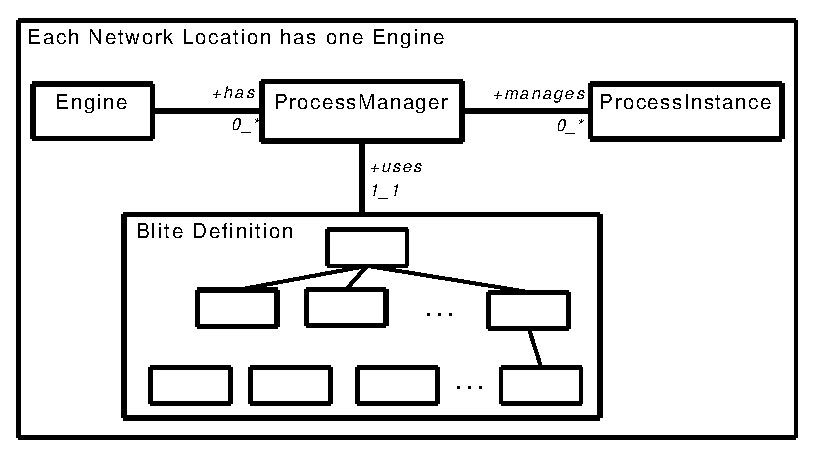
\includegraphics{architettura_interna/dia/engine}
%   \caption[]{
%   	\textsf{{\small Passaggio da reazioni a processi}}
%   }
  \label{fig:1}
\end{center}
\end{figure}

Per ogni definizione istallata sull'engine sarà presente un oggetto istanza
della classe \icode{ProcessManager}, che avrà il compito di gestire, nel loro
ciclo di vita, le istanze di processo derivate dalla definizione.

Prima di entrare nel dettaglio delle scelte architetturali ricapitoliamo quali
sono le caratteristiche peculiari di un sistema che deve gestire programmi per
l'orchestrazione di servizi, in modo che sia pi\`u facile da una parte
comprendere e dall'altra giustificare le scelte fatte.

A nostro vantaggio:
\begin{itemize}
  \item Un Engine contiene in generale un numero contenuto di definizioni, per
  cui non ci interessa la scalabilità rispetto alla quantità di definizioni
  istallate su singolo engine. Tale scalabilità al contrario può essere
  ottenuta aggiungendo altri engine e installando definizioni su engine diversi.
  
  \item  Una definizione (o programma) Blite avendo principalmente funzionalità
  di integrazione avrà una lunghezza generalmente limitata. 
  
  \item Poiché le operazione fondamentali di un programma di questo genere
  sono invocazioni remote, le durate delle esecuzioni hanno ordini di grandezza
  minimi dettati dai tempi caratteristici della rete. Per questo motivo non
  risulta determinante l'efficienza di esecuzione delle operazioni interne di un
  processo. Il nostro engine non necessiterà di una particolare ottimizzazione 
  rispetto all'efficienza di esecuzione interna.
\end{itemize}

al contrario risultano particolarmente critici i seguenti aspetti:
\begin{itemize}
  \item Per ciascuna definizione potrà essere richiesta la creazione di
  innumerevoli istanze. La scalabilità rispetto al numero delle
  richieste remote e quindi di istanze di processo risulta essere un
  prerequisito fondamentale.
  
  \item Se da un lato abbiamo detto che l'efficienza di esecuzione non \`e 
  una aspetto particolarmente critico, dall'altro per\`o ogni attività interna
  necessita di un elevato grado di controllo e tranciabilità. Ogni attività deve
  potere essere eventualmente terminata o abortita. Poiché in generale
  \footnotetext{} ogni istanza potrebbe avere un immagine persistente o
  perlomeno essere soggetta ad una attività di monitoring, l'engine necessiterà
  di un grado di controllo a livello di singola attività Blite.
\end{itemize}

Tenendo conto di queste iniziali considerazioni sono state fatte alcune scelte
basilari di organizzazione del progetto e l'architettura software \`e stata
basata sulle seguenti specifiche fondamentali:

\begin{enumerate}
  \item La compilazione di una definizione Blite (che eventualmente in un
  ambiente distribuito può essere fatta in fase di deploy) produce un modello
  statico della definizione stessa. Tale modello può essere implementato con una
  struttura ad oggetti che si può pensare di mantenere in memoria presso
  l'engine, tale struttura sarà navigata a runtime per ricavare il
  flusso e la logica di esecuzione. Sempre in fase di deploy l'engine può
  ricavare tutte le informazioni per popolare le strutture dati in cui sono 
  memorizzati i binding fra i nomi delle porte e le definizioni; anche tali
  strutture dati possono essere mantenute in memoria.
  
  \item Le richieste che giungono all'Engine non devono produrre un aumento
  delle risorse complessive mantenute dall'Engine. Ogni istanza di processo nel
  suo svolgersi deve, man mano che procede, rilasciare le risorse di memoria
  acquisite. Anche il numero dei thread complessivo deve essere limitato
  superiormente (generalmente dell'ordine dell'unita). La realizzazione del
  parallelismo di attività deve essere attuata tramite il pattern ``Resources
  Pool''. Ogni Engine deve disporre di un pool di thread con cui eseguire in
  parallelo le attività secondo le definizioni Blite.
  
  \item Il modello di esecuzione deve essere Activity Centric. L'engine deve
  trattare ogni attività secondo una astrazione generica che possa permettere di
  fattorizzare i comportamenti comuni e mantenere semplice e pulita
  l'implementazione della semantica di esecuzione del linguaggio.
\end{enumerate}

%%%%%%%%%%%%%%%%%%%%%%%%%%%%%%%%%%%%%%%%%%%%%%%%%%%%%%%%%%%%%%%%%%%%%%%%%%%%%%%%
%						Modello per l'Attività
%%%%%%%%%%%%%%%%%%%%%%%%%%%%%%%%%%%%%%%%%%%%%%%%%%%%%%%%%%%%%%%%%%%%%%%%%%%%%%%%
\section{Modello per l'Attività}
A questo punto dopo aver esposto a grandi linee quelle che devono essere le
caratteristiche fondamentali di un engine entriamo nel dettaglio del disegno
della architettura. Nella realizzazione di questa abbiamo scelto di utilizzare
il formalismo degli oggetti e delle classi secondo il consueto paradigma
``Object Oriented''. Inoltre abbiamo preso come fonte di
ispirazione il ``Composite Pattern'' [GANGo4] cercandone una trasposizione nella
problematica dell'esecuzione di un programma Blite. In particolare
l'astrazione di componente \`e stata applicata all'entità attività. Come i
componenti contribuiscono alla realizzazione di un documento o di una
interfaccia utente le singole attività contribuiscono allo svolgersi
dell'esecuzione del processo Blite.
 
Inoltre la tipica struttura gerarchica presente staticamente negli elementi
sintattici di una definizione può essere naturalmente riprodotta a runtime tra
i singoli step di esecuzione, andato a completare l'analogia con le strutture
gerarchiche ad albero tipiche dei tradizionali domini di applicazione del
Composite Pattern. 
\\

L'entità fondamentale del nostro dominio applicativo \`e stata quindi
individuata nella \icode{ActivityComponent} trasposizione a runtime
dell'elemento sintattico Activity definito dalla grammatica di Blite.
Ogni \icode{ActivityComponent} \`e rappresentabile tramite la seguente
interfaccia

\lstinputlisting
[caption={L'interfaccia base del modello di escuzione del Blite Engine},
label=lst:ActivityComponent]
{architettura_interna/java/ActivityComponent.java}

\begin{tabular}{| p{0.3\textwidth } | p{0.6\textwidth}|}
\hline
\icode{ActivityComponent} &  \\
\hline

\small{boolean \textbf{doActivity()}} & \small{\textsf{Costituisce il metodo
centrale per lo svolgersi dell'esecuzione del programma. L'invocazione di tale metodo su
un oggetto attività fa si che essa possa eseguirsi. Il valore booleano
ritornato sarà il discriminate del fatto che il flusso di esecuzione
corrente dovrà o meno interrompersi. Ogni attività oltre che eseguire se
stesa sarà quindi anche responsabile nel guidare il flusso nel passo
successivo. Utilizzando la gerarchia a lei nota imposterà la nuova attività
corrente da eseguire (l'attività padre o un figlio) e ritornerà il valore true. 
Al contraio potrà interrompere il flusso corrente ritornando false.
}}\\
 
& \\
\small{ActivityComponent \linebreak \textbf{getParentComponent()}} &
\small{\textsf{ Tale metodo restituisce se presente l'elemento padre 
dell'attività corrente. In questo modo si realizza la struttura gerarchica fra
i veri componenti dell'esecuzione. }}\\

& \\
\small{BltDefBaseNode \linebreak {\textbf{ getBltDefNode()}}} &
\small{\textsf{ Ogni attività componente dell'esecuzione \`e strettamente 
associata ad un elemento sintattico del programma. Con questo metodo ogni 
oggetto attività restituisce il nodo che la definisce nell'albero sintattico
ricavato dal parsing del codice Blite. }}\\

\hline
\end{tabular}


Lo scenario che si va a delineare \`e quindi quello di due strutture gerarchiche
associate: una costituita dall'AST (Abstract Syntax Tree) ricavato dal
parsing del codice Blite, e che come si detto \`e mantenuta nella sua interezza,
l'altra costituita dall'albero dinamico delle ActivityComponent che
realizzano l'esecuzione a runtime. Quest'ultima struttura, una per ogni
istanza, non \`e pero costruita in un unico momento in fase di inizializzazione
del  processo, ma al contrario \`e istanziata man mano che l'esecuzione
procede.  Come già accennato le attività stesse saranno responsabili di creare
i loro successori e di metterli in esecuzione. Inoltre gli oggetti attività
già eseguiti dovranno essere rilasciati il prima possibile in modo da poter 
essere collezionati dal Garbage Collector e rilasciare le risorse di memoria.

\begin{figure}[!htp]
\begin{center}
  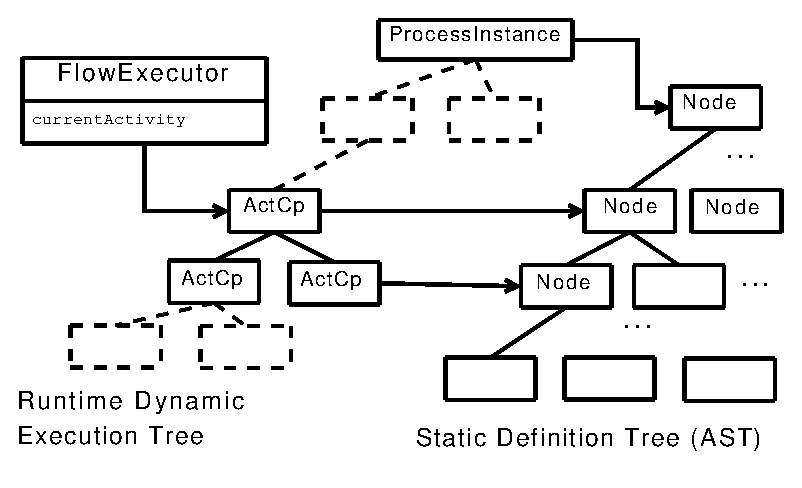
\includegraphics{architettura_interna/dia/tries}
%   \caption[]{
%   	\textsf{{\small Passaggio da reazioni a processi}}
%   }riscrivera
  \label{fig:1}
\end{center}
\end{figure}

Per ogni tipologia di attività prevista dalla grammatica di Blite esisterà
una sotto classe specifica implementante l'interfaccia \icode{ActivityComponent}
e che realizzerà in maniera opportuna, in rispetto della semantica, il metodo
\icode{boolean \textbf{doActivity()}}. Per ottimizzare il disegno e fattorizzare
il codice comune \`e stata ovviamente introdotta una classe astratta
\icode{ActivityComponentBase} da cui ogni altra implementazione di
\icode{ActivityComponent} erediterà le funzionalità comuni di base.

Anche la classe \icode{ProcessInstance}, che modellerà con i suoi oggetti le
varie istanze di processo nell'engine, implementerà l'interfaccia
\icode{ActivityComponent} uniformando la struttura gerarchica di esecuzione.

Le varie istanze di \icode{ActivityComponent} del tipo specializzato verranno
create tramite una classe di Factory \icode{ActivityComponentFactory} che
espone il FactotyMathod \icode{ActivityComponent
\textbf{makeRuntimeActivity}(BltDefBaseNode bltDefNode,\ldots )} 

\lstinputlisting
[caption={ActivityComponentFactory la factory per le ActivityComponent},
label=lst:ActivityComponentFactory]
{architettura_interna/java/ActivityComponentFactory.java}

\begin{center}
\begin{tabular}{| p{0.5\textwidth } | p{0.4\textwidth}|}
\hline
\icode{ActivityComponentFactory} & \\
\hline

\small{
ActivityComponent \linebreak \textbf{makeRuntimeActivity}( 
\linebreak \hspace*{\stretch{3}} BltDefBaseNode bltDefNode, 
\linebreak \hspace*{\stretch{3}} ExecutionContext context, 
\linebreak \hspace*{\stretch{3}} ActivityComponent parentComponent, 
\linebreak \hspace*{\stretch{3}} FlowExecutor executor)} 
& \small{\textsf{ Permette di ottenere istanze opportune di oggetti
\icode{ActivityComponent}. Il parametro bltDefNode individua l'elemento
sintattico che definisce l'attività specifica, in pratica il nodo nel AST.
Il parametro parentComponent l'attività padre nella gerarchia di esecuzione,
mentre gli altri due parametri individuano rispettivamente il contesto di
esecuzione e l'esecutore del flusso in cui l'attività verrà creata. Tali
entità verranno descritte nelle sezioni successive}}\\
\hline
\end{tabular}
\end{center}

In Figura \ref{fig:actclass} viene riportato un diagramma di classe
abbastanza dettagliato per le entità \icode{ActivityComponent}.

\begin{figure}[p]
\begin{center}
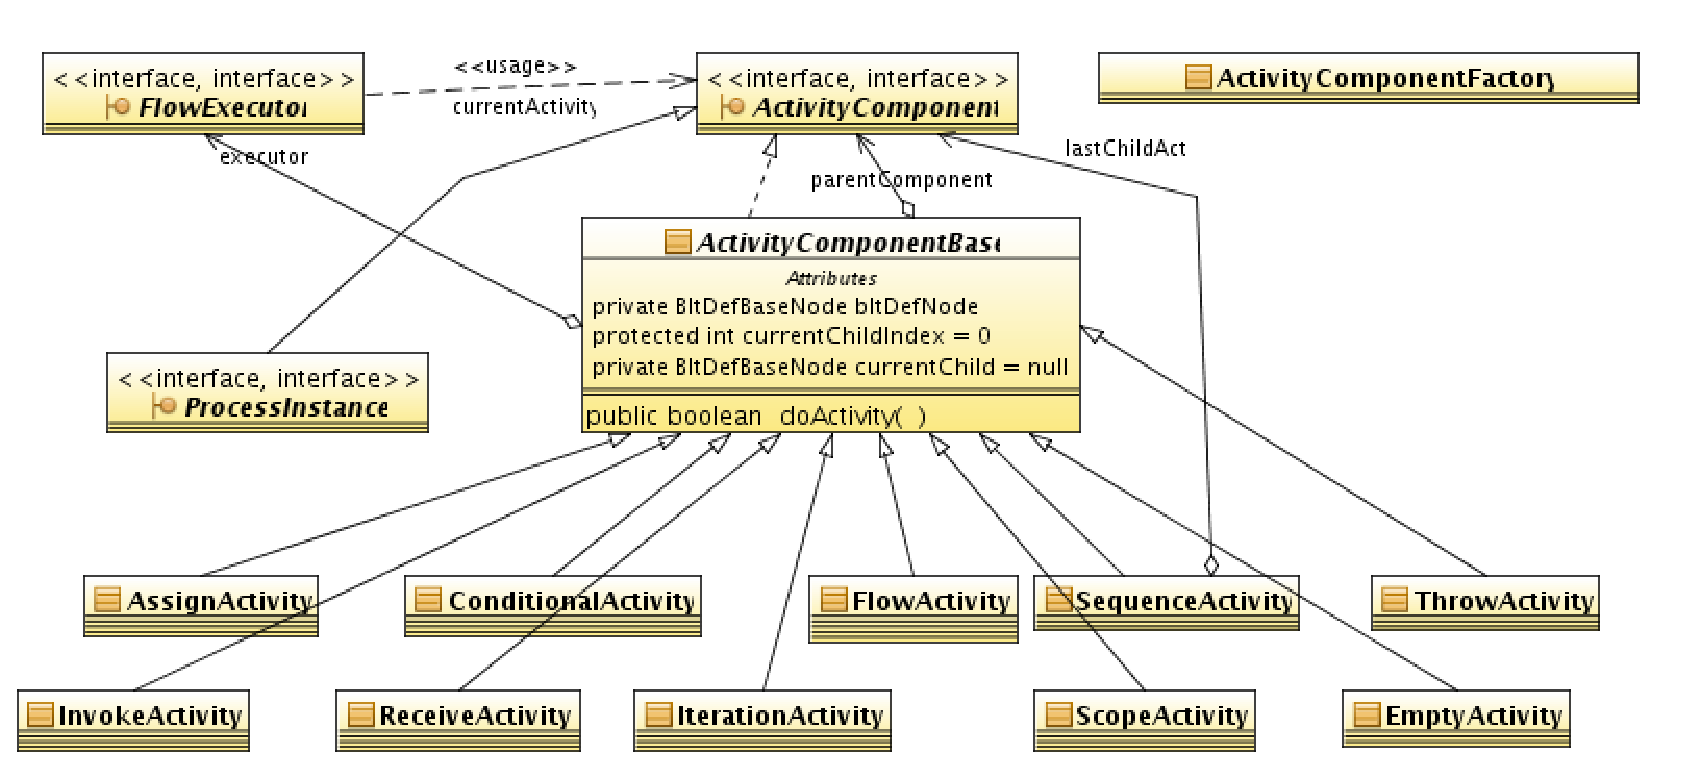
\includegraphics[angle=90,scale=0.80]
{architettura_interna/dia/actclass}
\caption[Gerarchia delle ActivityComponent]{
   	\textsf{{\small Diagramma di classe per la gerarchia delle
   	ActivityComponent}} }
  \label{fig:actclass}
\end{center}
\end{figure}

% %%%%%%%%%%%%%%%%%%%%%%%%%%%%%%%%%%%%%%%%%%%%%%%%%%%%%%%%%%%%%%%%%%%%%%%%%%%%%%%
% Esecuzione e parallelismo
% %%%%%%%%%%%%%%%%%%%%%%%%%%%%%%%%%%%%%%%%%%%%%%%%%%%%%%%%%%%%%%%%%%%%%%%%%%%%%%%
\section{Esecuzione e parallelismo}
Abbiamo visto come i componenti base per l'esecuzione siano oggetti delle varie
sottoclassi implementanti l'interfaccia \icode{ActivityComponent}, e come
l'esecuzione abbia atto tramite l'invocazione del metodo
\icode{\textbf{doActivity()}} su tali oggetti. A questo punto pero dobbiamo
domandarci da chi e in che modo tale metodo sia invocato. Nel rispondere a questa
domanda dobbiamo tenere conto che in un engine verranno eseguite
contemporaneamente molteplici istanze di processo e che inoltre il formalismo
stesso del linguaggio da la possibilità di richiedere l'esecuzione contemporanea
di diverse attività (costrutto flaw). Quindi su ciascun Engine dovranno essere
disponibili più thread per poter realizzare il sufficiente livello si
parallelismo.

Ovviamente si capisce bene che istanzire un nuovo oggetto Thread per ogni nuovo
flusso logico presente sull'engine non sia un approccio assolutamente
vantaggioso. Come già accennato infatti tale politica non sarebbe per nulla
scalabile rispetto al numero delle richieste remote gestite dell'engine; inoltre,
poiché ogni istanza di processo tendenzialmente trascorrerà la gran parte del suo
tempo in attesa di comunicazioni remote\footnote{Come già osservato i tempi di
comunicazione remota sono di ordini di grandezza molto maggiori rispetto alle
operazioni interne per cui ogni istanza nel suo ciclo di vita si troverà ad
occupare realmente la CPU per tempi quasi infinitesimi rispetto ai tempi di
attesa di eventi remoti}, ci troveremmo con un gran numero di thread in stato di
attesa, con un del tutto ingiustificabile spreco di risorse. Più banalmente
gestire direttamente oggetti Thread \`e un pratica alquanto sconsigliabile
\footnote{Questo \`e ancor pi\`u vero dalla versione 5 in poi di Java, in cui
sono stato introdotti i pacchetti \texttt{java.util.concurrent.*} che mettono a
disposizione un framework ad alto livello che ottimizza e astrae l'uso delle API
a più basso livello per la concorrenza}, in quanto può portare ad errori di
programmazione o ad Memory Leaks nel caso in cui il ciclo di vita di tali oggetti
non sia sempre ben condotto dal programmatore. Per queste motivazioni si \`e
scelto di utilizzare la tecnica del Pooling per gestire un insieme di Thread a
livello di Engine. Con tale tecnica si isola la gestione della tecnologia di
multitasking e si possono applicare politiche anche molto raffinate capaci di
adattare la quantità di risorse utilizzate al carico di lavoro da svolgere. Nella
implementazione attuale dell'Engine si \`e fatto uso dei thread pool forniti
dalla classe \texttt{java.util.concurrent.Executors} presente nella piattaforma
standard Java 5
 
La scelta che quindi \`e stata fatta per realizzare il sufficiente grado di
parallelismo \`e la seguente: ogni flusso logico attivo presente nelle varie istanze di
processo sarà associato all'entità \icode{FlowExecutor} (tale entità \`e già
comparsa in alcuni diagrammi precedentemente illustrati in questo capitolo, per
cui il lettore avrà già intuito la sua funzionalità). Tali oggetti
presenteranno un'interfaccia che permetterà da un lato di impostare l'attività corrente che
dovrà essere eseguita da uno dei thread del pool, dall'altro di eseguire
effettivamente tale attività.

\lstinputlisting
[caption={I FlowExecutors saranno gli oggetti che realizzeranno i flussi di
esecuzione parallela all'interno dell'Engine }, label=lst:FlowExecutor]
{architettura_interna/java/FlowExecutor.java}

A questo punto quando ci sarà bisogno di creare un nuovo flusso di esecuzione per
l'ActivityComponent \texttt{act} si dovrà creare un nuovo FlowExecutor settarci
\texttt{act} come attività corrente e renderlo disponibile ad un thread per
l'esecuzione. Questo ultimo passaggio verrà realizzato tramite l'interfaccia
dell'Engine che disporrà di un metodo per notificare gli executor pronti per
essere eseguiti e metterli a disposizione del pool di threads

\lstinputlisting {architettura_interna/java/queueFlowExecutor.java}

Inoltre ogni flusso giungerà a conclusione (un istanza di processo termina o un
esecuzione parallela definita in una flow Activity si conclude) e tale evento
dovrà essere registrato e produrre eventualmente altri effetti. Per far si che si
realizzi questa necessità si \`e introdotto il concetto di \icode{FlowOwner}.
Ogni attività che nel suo eseguirsi si troverà a creare nuovi flussi di
esecuzione e quindi oggetti \icode{FlowExecutor}  dovrà implementare
l'interfaccia \icode{FlowOwner} e settare se stessa nel FlowExecutor da lei
creato. In questo modo quando il flusso logico terminerà il FlowOwner potrà
essere notificato di tale accadimento tramite l'invocazione del metodo
\icode{flowCompleted()}.

\lstinputlisting
{architettura_interna/java/FlowOwner.java}

A questo punto \`e lecito domandarsi quando si dovrà considerare terminato un
flusso di esecuzione. In generale si applica il seguente ragionamento. Le varie
\icode{ActivityComponent}, che sono legate in una struttura gerarchica che
riflette la definizione statica del programma, termineranno la loro esecuzione
mettendo come attività corrente nel loro FlowExecutor la propria attività padre
(parentComponent). In accordo con questa osservazione risulta quindi corretto
affermare che flusso di esecuzione può essere considerato terminato dal
FlowExecutor quando questo si troverà ad eseguire come attività corrente proprio
il suo FlowOwner. In questo caso su di esso il FlowExecutor non dovrà invocare il
metodo doActivity() ma il metodo flowCompleted() e fatto questo, dovrà terminare
di eseguire il flusso. Il codice seguente spiega meglio di mille parole la logica
alla base di tutto il modello di esecuzione del Blite Engine; in poche righe \`e
sintetizzata il cuore dell'architettura

\lstinputlisting{architettura_interna/java/FlowExecutorImp.java}

In generale possiamo quindi dedurre le seguenti affermazioni che ci possono
aiutare a sintetizzare delle proprietà invarianti

\begin{itemize}
  \item Un FlowExecutor non invocherà mai il metodo doActivity() del suo
  FlowOwner. Viceversa di questo invocherà prima o poi il metodo
  flowCompleted().
  
  \item Su un oggetto ActivityComponent che implementa anche l'interfaccia
  FlowOwner, il metodo doActivity() verrà invocato dal FlowExecutor dell'attività 
  padre.
  
  \item Su di un oggetto ProcessInstance, che \`e il FlowOwner del flusso
  principale dell'istanza e che \`e l'unica attività senza padre, 
  il metodo doActivity() non verrà mai invocato da nessun FlowExecutor.
  
  \item il metodo doActivity() di una ProcessInstance verra' invocato
  dell'Engine stesso in fase di creazione dell'istanza.
  
\end{itemize}

Oltre a creare, eseguire e terminare flussi sarà anche necessario sospenderne
alcuni già in esecuzione, vedi per esempio il caso dell'attività di ricezione
che deve fermare il flusso corrente in attesa di un evento remoto. In questo
caso l'attività utilizzando l'interfaccia dell'Engine e in particolare il
seguente metodo

\lstinputlisting{architettura_interna/java/addFlowWaitingEvent.java}

potrà mettere in attesa il suo FlowExecutor su di un evento identificato dalla
chiave \texttt{eventKey} e che lei stessa aveva provveduto
precedentemente a creare. Fatto questo l'attività ritornerà dal proprio metodo
doActivity() con il valore false, in questo modo il FlowExecutor terminerà
l'esecuzione del Flow corrente. Nel momento in cui il messaggio sarà recapitato,
l'Engine potrà individuare il FlowExecutor tramite la chiave \texttt{eventKey} e
rimetterlo in esecuzione, poiché l'attività corrente di quest'ultimo sarà rimasta
l'attività di ricezione essa potrà riprendere il suo lavoro, consumando il
messaggio e permettendo al suo flusso di esecuzione di continuare. Nella sezione
successiva verrà illustrato nel dettaglio come si realizza la comunicazione e la
notifica degli eventi.

In Figura \ref{fig:flowclass} \`e rappresentato un diagramma di classe che
raffigura fra le altre l'entità il FlowExecutor e FlowOwner e le principali
relazioni che le coinvolgono.

\begin{figure}[p]
\begin{center}
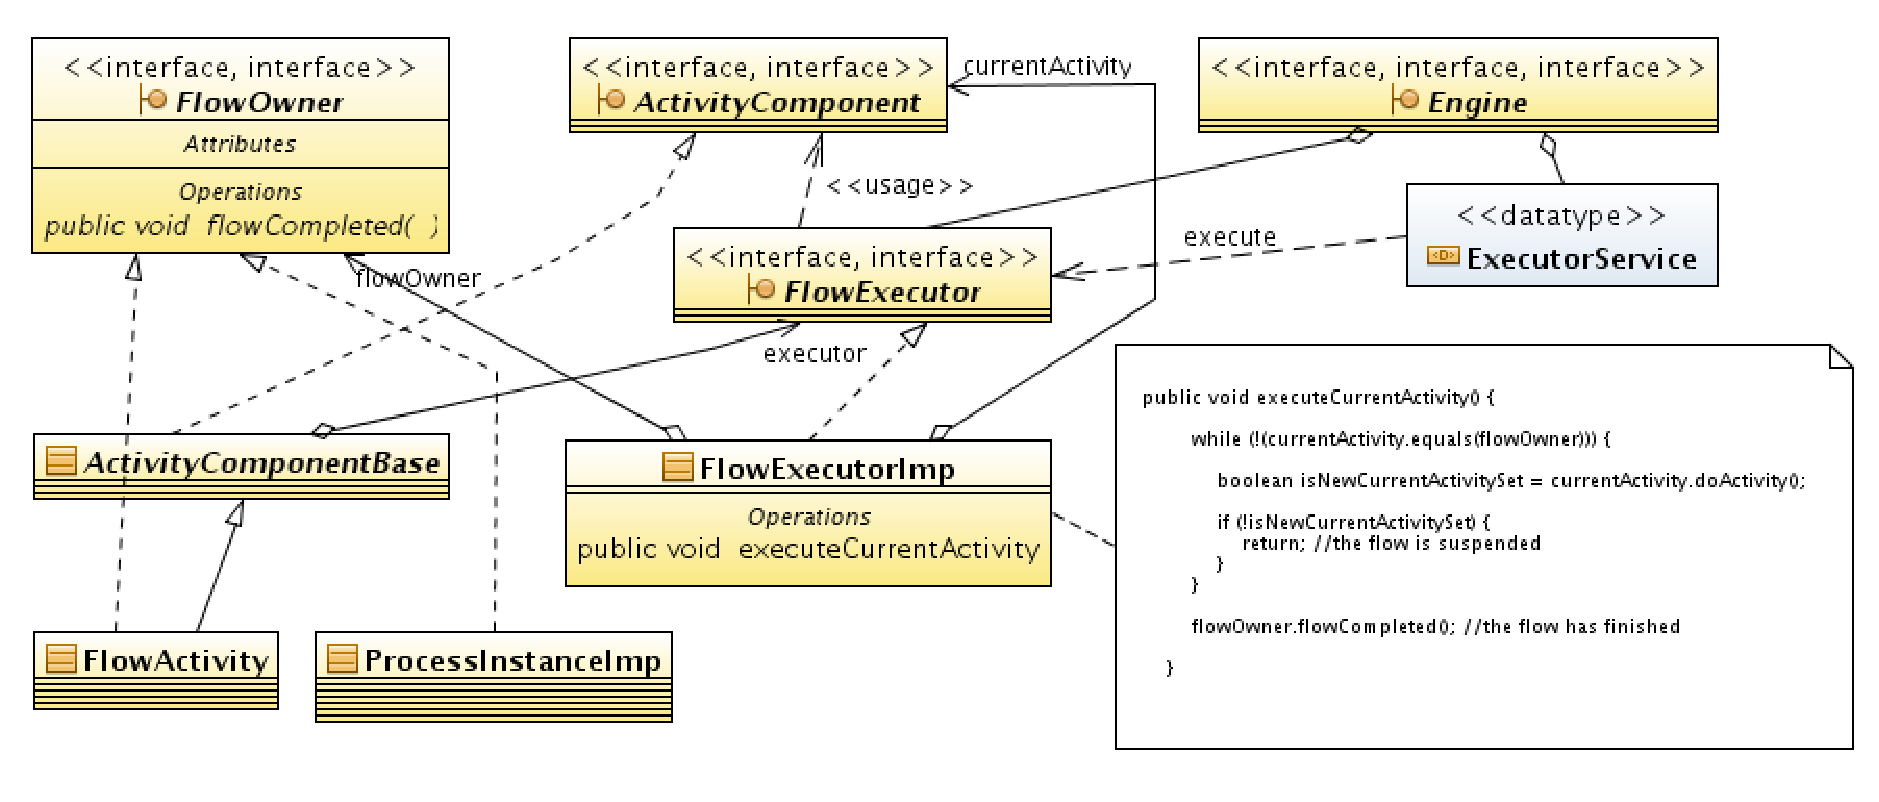
\includegraphics[angle=90,scale=0.75]
{architettura_interna/dia/flowClassDiagram}
\caption[Diagramma di classe FlowExecutor \ldots] {
   	\textsf{{\small Diagramma di classe FlowExecutor, FlowOwner e ThreadPool}} }
  \label{fig:flowclass}
\end{center}
\end{figure}

% %%%%%%%%%%%%%%%%%%%%%%%%%%%%%%%%%%%%%%%%%%%%%%%%%%%%%%%%%%%%%%%%%%%%%%%%%%%%%%%
% EVENTI E COMUNICAZIONE
% %%%%%%%%%%%%%%%%%%%%%%%%%%%%%%%%%%%%%%%%%%%%%%%%%%%%%%%%%%%%%%%%%%%%%%%%%%%%%%%
\section{Comunicazione ed eventi}
Da quanto abbiamo già esposto risulta chiaro che l'esecuzione di un processo \`e
caratterizzata da lo svolgersi di attività interne e l'accadere di eventi
esterni di cui l'attività possono essere in attesa. In generale si può
considerare che gli eventi si generino a livello di Enviroment, e che possano
essere prodotti dall'arrivo di nuovi messaggi verso alle porte locali o
dalla notifica degli acknologment delle invocazioni locali
verso porte remote. Attualmente le funzionalita' espresse da Blite non
individuano eventi diversi da queste due tipologie. Nelle engine pero' si \`e
preferito realizzare un meccanismo generico di notifica di eventi che
soddisfacesse i requisiti attuali del linguaggio ma che non escludesse eventuali
possibilità di estensione verso altre caratteristiche tipiche di BPEL
(comunicazione Request-Response, EventActivity, ecc).

Per l'implementazione dello schema di comunicazione prescelto saranno richieste
le seguenti funzionalita'

\begin{enumerate}
  \item A livello di attvita' o di ProcessManager stesso,
  sara' necessario ricavare una chiave univoca per uno specifico 
  evento\footnote{Si usa qui il termine ricavare e non generare in maniera
  voluta. Le chiavi di evento non sono identificati da oggetti in memoria ma hanno una loro entita' indipendete
  dagli oggetti che posso essere creati per rappresentarle.}.
  I tipi di evento e le regole per generare di volta in volta 
  le chiavi verrano esposti di seguito. Per il momento puo' bastare aver 
  chiaro che una chiave individua in maniera univoca una particolare 
  tipologia di evento e all'interno di questa un evento specifico o un insieme
  di eventi gemelli. 
  
  \item In un qualsiasi momento al ProcessManager potranno essere notificati
  eventi. In tal caso esso dovrà provvedere a ricavarsi la chiave e a
  memorizzare associativamente l'evento alla chiave per poterlo poi rendere
  disponibile all'attivita' interessate. Il ProcessManager dovrà anche
  provvedere a ``risvegliare'' tutti i flussi di esecuzione che
  eventualmente si sono messi in attesa di quel evento specifico.
   
  \item In un qualsiasi momento e anche più volte nel suo ciclo di vita una
  Attività potrà interrogare l'Engine (o meglio il ProcessManager responsabile
  della sua istanza) chiedendogli se un evento associato ad una particolare
  chiave sia avvenuto. In caso affermativo l'attività potrà consumare l'evento.

  \item Una attività potrà avere la necessità di mettersi in attesa di un
  particolare evento non ancora avvenuto, il tal caso dovrà sospendere il
  suo flusso di esecuzione e notificare questo al ProcessManager
  associativamente alla chiave dell'evento d'interesse. 
\end{enumerate}

Tali funzionalità serrano rese disponibili nelle diverse interfacce 


\ldots
\\

In particolare si può vedere come queste funzionalità di base possano essere
utilizzate nel caso dell'attività \icode{ReceiveActivity}, e come
l'attività stessa collabori con il ProcessManager perché si realizzi la
ricezione di messaggi. La \icode{ReceiveActivity} nel suo metoto doActivity
compiera' i seguenti passi logici:

\begin{enumerate}
  \item Si ricava la chaive d'evento \texttt{eventKey}. In questo caso
  particolare la chiave sara' di tipo \icode{RequestInComingEventKey} e la sua
  unicita' sara costituita dal \texttt{portId} ( ovvero la coppia 
  serviceName/operationName) delle porta su cui si sta eseguendo l'operazione di 
  ricezione. Ovviamente la ReceiveActivity potra' ricavare il \texttt{portId}
  dal nodo della definizione sitattica a lei associata.
  
  \item Si richiede al ProcessManager il set degli eventi associati alla
  \texttt{eventKey}. Se non c'e' alcun evento associato si mette in attesa il
  FlowExecutor sull'evento \texttt{eventKey}, si termina ritornando
  \texttt{false}.
  
  \item Si analizza il set degli eventi (che in questo caso possono essere
  identificati con tutti messaggi indirizzati alla porta in questione non
  ancora consumati) per vedere se ce ne possa essere uno indirizzabile alla
  instanza della ReceiveActivity in questione. Questo controllo \`e fatto in
  base alle regole di correlazione. Se un tale messaggio non viene identificato
  si mette in attesa il FlowExecutor sull'evento \texttt{eventKey} e si termina
  ritornando \texttt{false}. 
  
  \item Si \`e individuato un messaggio inviato alla porta e alla istanza in
  questione. Si consuma tale messaggio aggiornando lo stato delle variabili
  conivolte nella ricezione, si imposta la parentComponet come attivita'
  corrente del FlowExecutor si termina ritornando \texttt{true}.
\end{enumerate}

Daltro canto un oggetto ProcessManager nel metodo \icode{manageRequest( 
ServiceIdentifier service, String operation, MessageContainer
messageContainer)}\footnote{Bisogna notare che
l'invocazione di tale metodo sara' scatenata lato Environment, e che la sua
esecuzione avverra' a carico di un Thread allocato a livello stesso di
Environment logicamente del tutto indipendente dai thread del pool
dell'Engine} eseguira le seguenti operazioni:

\begin{enumerate}
  \item Si verifica che la terna serviceName/operationName/numero parti del
  messaggio identifichi effettivamente una porta valida per la definizione 
  di processo in questione. Se non \`e cosi si notifica una
  situazione di errore all'Enviroment e questo provvedera' ad inviare un NOK al
  processo invocante.
 
 \item Si ricava il RequestInComingEventKey \texttt{eventKey} associata alla
 porta e con questa si provvede a memorizzare il messaggio in arrivo in una mappa associativa.
 
 \item Se la porta in questione individua una start activity si crea una nuova
 istanza di processo e la si mette in esecuzione, alternativamente 
 
 \item Se la porta non \`e associata ad una start activity si risvegliano tutti
 i FlowExecutor in attesa di eventi individuati dalla \texttt{eventKey}.
\end{enumerate}

Gia' pensando che le due procedure precedenti saranno eseguite concorrentemente
si capisce che un punto particolarmente critico del meccanismo di
notifica/consumo di eventi sta nel fatto che l'elevato grado di parrallelismo
presente possa portare ad una perdita eventi (ovvero non consegna di messaggi).
Quest'ultima \`e di fatto un ipotesi assolutamente inammisibile e che deve essere
assolutamente evitata. Di fatto essa si manifesterebbe allorche il parallelismo
delle fosse sequenzializzato per esempio nel seguente modo

% %%%%%%%%%%%%%%%%%%%%%%%%%%%%%%%%%%%%%%%%%%%%%%%%%%%%%%%%%%%%%%%%%%%%%%%%%%%%%%%
% CONTESTI E COMPESAZIONE
% %%%%%%%%%%%%%%%%%%%%%%%%%%%%%%%%%%%%%%%%%%%%%%%%%%%%%%%%%%%%%%%%%%%%%%%%%%%%%%%
\section{Contesti, FaultHandler e Compensazione}





% Blite
\include
%\chapter{Blide}

\textsf{
In questo capitolo viene presentato \emph{Blide} (Blite Integrated Development
Environment) un tool che racchiude un ambiente di esecuzione locale e
fornisce un intrefaccia grafica che permette di svolgere in maniera integrata
tutte le operazioni legate allo sviluppo di programmi Blite. Nella prima parte
del capitolo vengono descritte le caratteristiche e le funzionalità
dell'interfaccia, mentre nella seconda parte se ne presetano alcuni
esempi di utilizzo.
}

\section{Un IDE per Blite}

Oltre al motore di esecuzione si è realizzato un vero e proprio IDE per
sviluppare i programmi Blite. Questo strumento prevede la possibilità di
gestire i file con le definizioni dei processi, editarli, compilarli e metterli
in esecuzione. E' prevista anche la funzionalità per visualizzare, tramite una
rappresentazione grafica, l'esecuzione delle istanze di processo.

Blide è stato realizzato tramite la piattaforma \emph{NetBeans Platform}
[NBPlatSite], un framework studiato per facilitare lo sviluppo di applicazioni
Java con interfaccia grafica. E' stato scelto tale progetto per la sua
completezza e per il modello architetturale offerto. 

NetBeans Platform permette allo sviluppatore di realizzare le proprie
applicazioni componendo diversi moduli ciascuno dei quale offre una
funzionalità specifica.

\begin{figure}[b]
\begin{center}
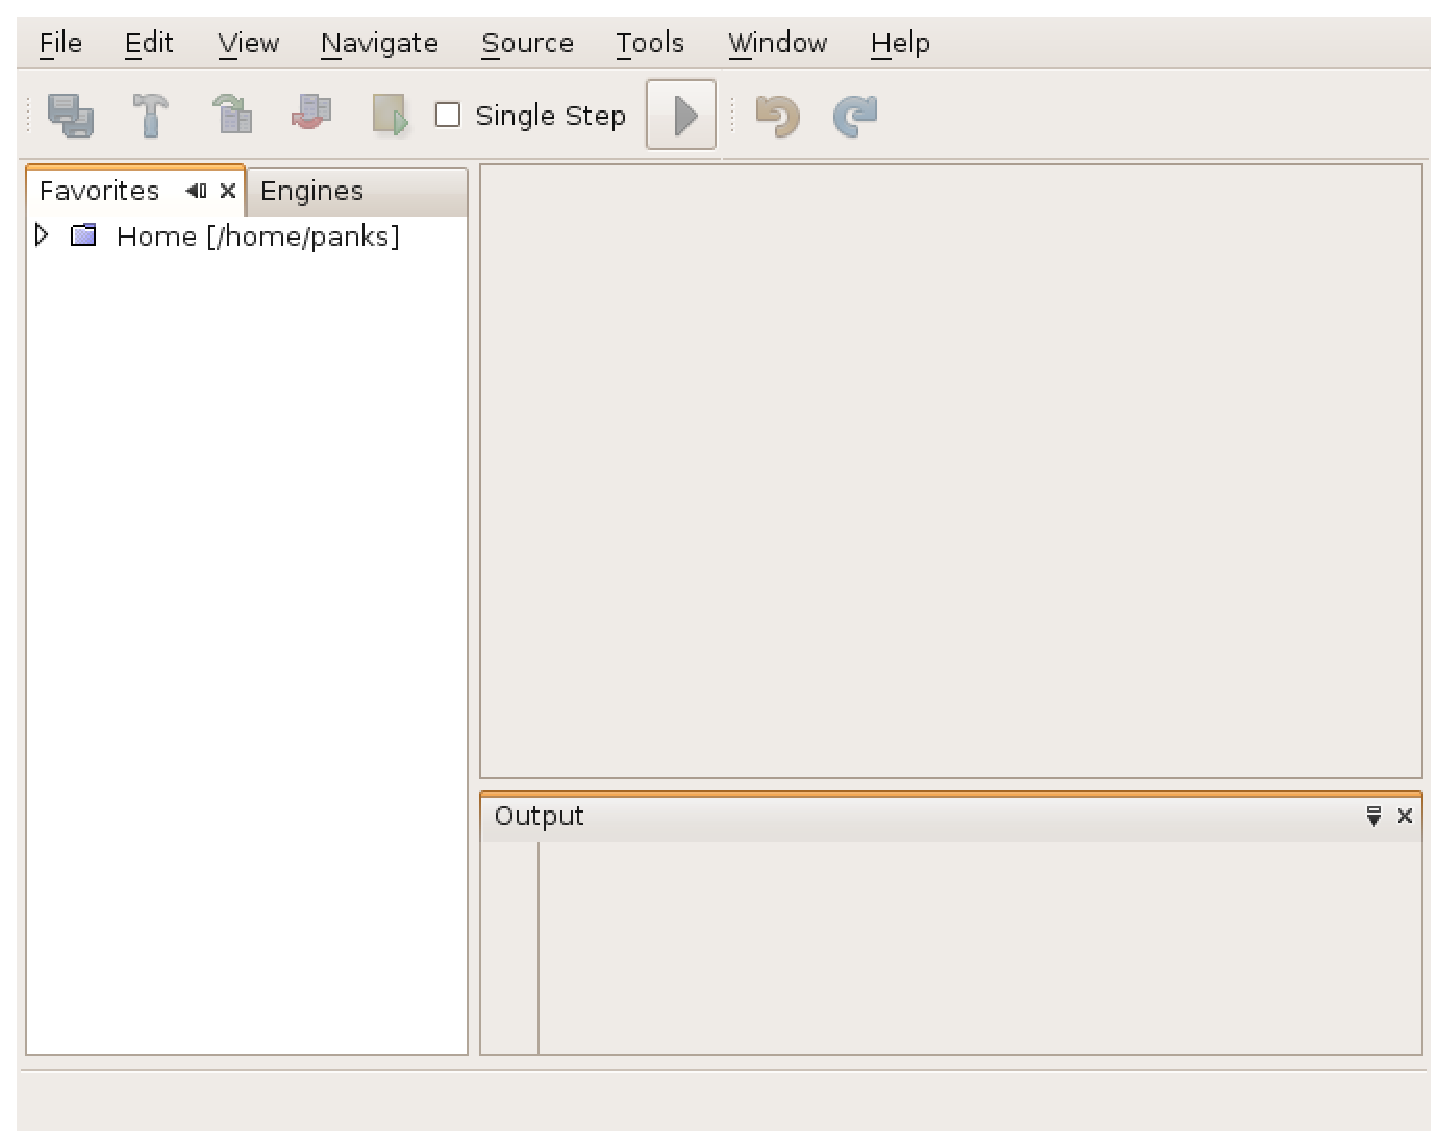
\includegraphics[scale=0.60]
{blide/dia/Blide1}
\caption[] {}
  \label{fig:blide1}
\end{center}
\end{figure}
 


% Blite
\include
%\chapter{Conclusioni e sviluppi}

\section{Osservazioni}


Realizzare un'implemetazione del linguaggio ci ha permesso di analizzare
approfonditamente la semantica formale definita per Blite e di capire quali
aspetti di essa risultassero particolarmente critici in fase di implementazione,
e più in generale ci permesso di fare alcune riflessione su BPEL e
sul significato di alcune sue funzionalità.
\\

Il lavoro svolto in questa tesi non è da considerarsi esaustivo
ma vorrebbe essere solamente l'inizio di un procedimento iterativo, il cui fine
dovrebbe essere quello di ottenere uno strumento funzionale per
l'orchestrazione di servizi, con una semantica rigorosa da cui sia possibile
ricavare implemetazioni coerenti. 

In particolare abbiamo capito che un linguaggio per l'orchestrazione di servizi,
come BPEL, risulta essere uno strumento molto complesso, e per questo
riuscirne a sintetizzare gli aspetti cruciali in una semantica formale è
veramente un'attività delicata. Contemporaneamente sviluppare una
implemetazione di tale semantica, in rispetto dei requisiti che ci possono
essere in sistemi di produzione, non è da meno complicato. 

Per questo può essere utile che le varie attività trovino sostegno reciproco.
Come l'implemetazione è guidata dalla semantica, così può essere utile che
l'esperienza ricavata dal processo di sviluppo ritorni nella fase di specifica
formale per apportare eventualmente revisioni e migliorie, e cosi
iterativamente fino al raggiungimento di un accettabile grado di funzionalità.
\\

% Realizzando l'implementazione abbiamo capito che potrebbe essere interessante
% a livello formale porre più enfasi sul sistema di correlazione, al fine di
% ridurre al minimo i conflitti che si possano creare nell'attribuzione dei
% messaggi alle diverse istanze di processo. 
% 
% In particolare potrebbe valere la pena di svincolare lo stato della correlazione
% dallo stato interno della memoria dei processi e di associarlo solamente alla
% comunicazione dell'informazione.

%Per esempio 
Un punto molto critico in cui la specifica della semantica è
risultata partiolarmente lontana dalle soluzioni implemetative è stato quello
in cui essa definisce la correlazione dei messaggi con le diverse istanze di
processo e risolve il problema delle \emph{multiple start activity}. In
particolare la sematica di Blite specifica tale comportamento in maniera molto
brillante e con un forlmalismo estremamente sintetico ed efficace, ma che mal
si presta a guidare lo sviluppo del software. 

In un'implemetazione che usa il \emph{multithreading} per realizzare il
parallelismo, non ha senso parlare di più istanze di processo che eseguono
contemporaneamente la ricezione sulla medesima porta, per cui diventa inutile
valutare una priorità nell'attribuzione dei messaggi alle diverse istanze.

Di fatto un'istanza di processo, nel momento in cui si trova nella condizione
di poter consumare un messaggio , può stabilire se questo è a lei
correlato semplicemente valutando la funzione booleana:

$$
\begin{array}{c}
\x{corr}(\xcorr, \xsigma, \xx, \xv	) =
\left\{
\begin{array}{l@{\hspace{2ex}}l}
\\[-.50cm]
false & \textrm{se}\ \xx \in \xcorr \, \wedge \, \xx \in \xdom{\xsigma} \xx \in
\xcorr\ \, \wedge \, \xv \neq \xsigma(\xx)
\\[-.05cm] true & \textrm{altrimenti} \\
\end{array}
\right.
\\[.7cm]
%\xxnewmatch{\xcorr}{\xsigma}{\xv}{\xv} =
%\emptyset \qquad
\x{corr}(\xcorr, \xsigma, \arr{}, \arr{}) =
\emptyset
\\[.7cm]
\prooftree
\x{corr}(\xcorr, \xsigma, \xx_1, \xv_1) = b'
\quad
\x{corr}(\xcorr, \xsigma, \bar{\xx}_2, \bar{\xv}_2) = b''
\justifies \
\x{corr}(\xcorr, \xsigma, (\xx_1,\bar{\xx}_2), (\xv_1,\bar{\xv}_2)) =
b' \wedge b''
\endprooftree
\\[.7cm]
\end{array}
$$


Se dal punto di vista dell'attribuzione dei messaggi alle istanze il problema
può considerarsi risolto, rimane il fatto di distinguere se un
messaggio in arrivo ne debba produrre o meno una nuova. Il
\icode{ProcessManager} deve di fatto prendere questa decisione al momento della
ricezione in base a le informazioni di cui dispone in quel momento. 

In generale si potrebbe pensare di risolvere semplicemente il problema a livello
sintattico\footnote{La soluzione può sembrare ingenua ma per esempio è ciò che
di fatto fa Oralce Process Manager.}, rendendo distinguibili le porte di
ricezione su cui vengono create le istanze (\emph{create port}). E' ovvio che questa tecnica non permetta di realizzare le multiple start
activity, in cui una porta è contemporaneamente di creazione e di possibile
correlazione. Per realizzare le multiple start activity ci deve essere un
flusso d'informazione che dalle istanze passa al \icode{ProcessManager} nel
momento in cui viene assegnato un valore ad una variabile producendo
l'istanziazione di uno \emph{stato di correlazione} associato ad una porta.

Con questa informazione il \icode{Process Manager} può sapere se esiste o meno
un'istanza in grado di correlare con un messaggio in arrivo ad una porta, e in
particolare per le multiple start activity può utilizzare tale informazione per
distinguere se trattare la porta come di creazione o di correlazione.

E' chiaro che la semantica attuale di Blite specifica alla perfezione il
comportamento voluto, ma crea un notevole scarto tra la sfera teorica e quella
tecnologica che rende difficile capire quanto l'implementazione realizzi del
tutto tale comportamento. Inoltre diversi processi di svluppo possono attuare
strategie di implemetazione tra loro completamente diversi aumentando di fatto
la probabilità di difformità.
  
\section{Sviluppi}

Nella direzione dello sviluppo software le attività da poter svolgere sono
essenzialmente due:

\begin{itemize}
  \item Sviluppare diversi Enviroment per l'Engine di Blite per realizzare
  diversi strategine di comunicazione.
  \item Migliorare il formalismo e la tecnologia grafica usata per la
  rappresentazione delle istanze in Blide.
\end{itemize} 

Per quanto riguarda il primo punto come già più volte detto le possibilità sono
molteplici. 

Un primo posso molto semplice potrebbe essere quello di creare un Environmet
che supporti la comunicazione remota fra programmi Blite. In questo caso si
potrebbe utilizzare una tecnologia nativa per implementare la comunicazione. Per
esempio utilizzando le socket e la Java Object Serialization si potrebbe di
fatto scambiare in rete gli oggetti attualmente utilizzati dal Local
Environment e avere quindi la possibilità di
distribuire i Deployment Blite su diversi nodi di rete. Ovviamente per poter
fare questo bisogna che ai nomi dei servizi sia associato un indirizzo di rete.

Questa associazione può essere fatta direttamente nel file di definizione di
Blite, in pratica la sintassi stessa delle invoke potrebe esplicitare
l'indirizzo dell'host a cui è diretto il messaggio


Alternativamente per non appesantire troppo la struttura del codice potrebbe
essere prevista una sezione a parte in cui si va a legare un nome simbolico utilizzato
nelle invoke con un indirizzo fisico.

Sicuramente molto più interessante sarebbe poter far dialogare i nostri
programmi Blite con altri tipi di servzi definiti con linguaggi e tecnologia
diversa, primi fra tutti i Web Service. Per far questo la cosa fondamentale è
creare un meccanismo che relazioni il codice Blite alle definizioni WSDL.

In pratica serve da una parte ricavare una definizione dell'interfaccia del
processo Blite, e dall'altra associare le operazioni d'invocazione ad alcune
definizioni di servizi presistenti.

Il processo di creazione dell'interfaccia può essere fatto per esempio
combinando un attività utente con un processo automatico.
Tramite un analisi del codice Blite si potrebbe pensare di creare uno
scheletro per la definizione WSDL che poi l'utente possa successivamente
raffinare andando per esempio ad esplicitare i tipi XSD delle parti dei
messaggi, alcuni riferimenti dei nemaspace o alcuni dettagli del bainding
WSDL/SOAP. In questo modo non ci sarebbe ovviamente nessun controllo statico che
i messaggi ricevuti siano usati all'interno del codice Blite in maniera conforme
con il tipo esplicitato nel contratto, ma questo concorda con la gestione
attuale in cui a runtime si attua una conversione implicita dei tipi o se in
ultima analisi nessuna conversione è applicabile si genera un errore.

L'associazione delle operazioni di output con le definizioni WSDL dei servizi
partner può essere fatta inserendo alcune meta annotazioni nel codice Blite
associando per esempio i nomi dei servizi alla coppia
$\langle$service:name/port:name$\rangle$

Una volta che si dispone di un meccanismo che permetta di legare i programmi Blite
alla tecnologia WSDL, la realizzazione di un Environment che supporti JBI si
riduce a operazioni di manipolazione di XML, in quanto è sufficente mettere a
punto dei traduttori che dalla specifica delle interfaccia del programma Blite 


Per quanto riguarda Blide le







% Riferimenti
\include
%\begin{thebibliography}{}

[LaPuTie1]
\\

[OASISSite]
\\

[XML]
\\

[XMLSchema]
\\

[WSDL]
\\

[SOAP]
\\

[Java]
\\

[JavaCC]
\\

[JJTree]
\\

[JBI]
\\

[NBPlatSite] NetBeans Platform Web Site
\\

[ContxSensWikiPedia] Pagina di riferimento per la definizione Context-Sensitive
Interface
\\

[GLFSite] Generic Languages Framework (GLF) Site	
\\

[GANGo4]
\\

[IMC]
\\


[RichClientApp] Geertjan Wielenga, Jaroslav Tulach and Tim Boudreau
\emph{``Rich Client Programming: Plugging into the NetBeans Platform ''} 2007
Sun Press. ISBN 0132354802
\\

[SVN]
\\

[GCode]
\\

[GPLv3]
\\

\end{thebibliography} 

\end{document}
